\documentclass[czech,bachelor]{diploma}

\usepackage[autostyle=true,czech=quotes]{csquotes}
\usepackage[backend=biber, style=iso-numeric, alldates=iso]{biblatex}
\addbibresource{sources.bib}
\usepackage{dcolumn}
\usepackage{subfig}
\usepackage[cpp]{diplomalst}
\usepackage{chngcntr}
\usepackage{float}
\usepackage{array}
\usepackage{tikz}
\usepackage{listings}

\usetikzlibrary{positioning}
\lstdefinelanguage{JavaScript}{keywords={function, return, var, let, const, if, else, for, while, do, break, continue, switch, case, default, new, this, typeof, true, false, null, undefined}, keywordstyle=\bfseries, sensitive=true, comment=[l]{//}, morecomment=[s]{/*}{*/}, commentstyle=\itshape, morestring=[b]", morestring=[b]', stringstyle=\ttfamily}

\ThesisAuthor{Martin Dressler}
\ThesisSupervisor{Ing. Martin Kot, Ph.D.}
\CzechThesisTitle{Komponenta výukového serveru TI - Amortizovaná složitost 1}
\EnglishThesisTitle{Component of Teaching Server for Theoretical Computer Science - Amortized~Complexity 1}

\SubmissionYear{2026}
\ThesisAssignmentFileName{DRE0065_BP.pdf}

\Acknowledgement{Rád bych poděkoval vedoucímu mé bakalářské práce Ing. Martinu Kotovi, Ph.D. za odborné vedení, cenné rady, trpělivost a čas, který mi věnoval při zpracování této práce. Zároveň mu děkuji za možnost věnovat se tématu, které může přispět k lepšímu pochopení amortizované složitosti budoucím studentům.}

\CzechAbstract{Tato bakalářská práce se zabývá problematikou amortizované složitosti. Cílem praktické části bylo vytvořit komponentu výukového serveru pro předmět Teoretická informatika v navazujícím magisterském studiu. Výsledná aplikace má podobu dynamické webové stránky, která vizualizuje vybrané algoritmy vhodné pro analýzu amortizované složitosti a umožňuje uživateli pracovat s různými typy vstupů. Součástí aplikace je zobrazení jednotlivých kroků algoritmů, změn stavů datových struktur a dalších hodnot důležitých pro pochopení jejich chování. Teoretická část se věnuje vysvětlení amortizované složitosti, souvisejících pojmů a metod, popisu implementace vytvořené komponenty a charakteristice vybraných algoritmů. Výsledkem práce je výukový nástroj, který může přispět k~lepšímu pochopení amortizované složitosti studenty.}

\CzechKeywords{Amortizovaná složitost; potenciální metoda; vizualizace algoritmů; výukový server; teoretická informatika; webová aplikace; HTML5; CSS3; JavaScript; Bootstrap}

\EnglishAbstract{This bachelor's thesis deals with the issue of amortized complexity. The goal of the practical part was to create a component of a teaching server for the course Theoretical Computer Science in~the~follow-up master's degree programme. The resulting application takes the form of a dynamic web page that visualizes selected algorithms suitable for amortized complexity analysis and allows the user to work with different types of inputs. The application includes the display of individual algorithm steps, changes in the states of data structures, and other values important for understanding their behavior. The theoretical part focuses on the explanation of amortized complexity, related concepts and~methods, the description of the implementation of the created component, and~the~characteristics of the selected algorithms. The result of the thesis is an educational tool that can contribute to a better understanding of amortized complexity by students.}

\EnglishKeywords{Amortized complexity; potential method; algorithm visualization; teaching server; theoretical computer science; web application; HTML5; CSS3; JavaScript; Bootstrap}

\AddAcronym{API}{Application Programming Interface}
\AddAcronym{BST}{Binary Search Tree}
\AddAcronym{CSS}{Cascading Style Sheets}
\AddAcronym{DOM}{Document Object Model}
\AddAcronym{FIFO}{First In, First Out}
\AddAcronym{HTML}{HyperText Markup Language}
\AddAcronym{HTTP}{HyperText Transfer Protocol}
\AddAcronym{JS}{JavaScript}
\AddAcronym{LIFO}{Last In, First Out}
\AddAcronym{PDF}{Portable Document Format}
\AddAcronym{TI}{Teoretická informatika}
\AddAcronym{UI}{User Interface}
\AddAcronym{UML}{Unified Modeling Language}
\AddAcronym{URL}{Uniform Resource Locator}

\newcolumntype{d}[1]{D{,}{,}{#1}}
\newcolumntype{L}[1]{>{\raggedright\arraybackslash}p{#1}}
\counterwithin{figure}{section}
\counterwithin{table}{section}
\setcounter{tocdepth}{2}
\raggedbottom
\begin{document}

\MakeTitlePages

\listoffigures
\clearpage

\listoftables
\clearpage

\chapter{Úvod}
Hlavním cílem této bakalářské práce bylo vytvoření komponenty pro výukový server v oblasti teoretické informatiky. V praktické části bylo potřeba navrhnout a implementovat dynamickou webovou aplikaci, která by sloužila jako názorný a interaktivní nástroj pro pochopení vybraných algoritmů a principů amortizované složitosti. Výsledná aplikace má studentům umožnit sledovat průběh jednotlivých operací, změny stavů datových struktur a další důležité hodnoty potřebné pro lepší pochopení chování algoritmů i jejich amortizované složitosti.

Problematika amortizované složitosti patří mezi velmi důležitá témata při studiu algoritmů a datových struktur. Její význam spočívá v tom, že umožňuje lépe popsat chování algoritmů v situacích, kdy jednotlivé operace nemají vždy stejnou cenu a jejich skutečná náročnost se projeví až v rámci delší posloupnosti kroků. U některých algoritmů a datových struktur nestačí hodnotit jednotlivé operace samostatně, protože jejich skutečná efektivita se ukáže teprve při sledování delší posloupnosti operací.

I když je amortizovaná složitost významnou součástí TI, bývá pro mnoho studentů obtížně pochopitelná. Hlavním důvodem je její abstraktnější charakter, protože při snaze o její pochopení nestačí sledovat pouze výsledek jedné operace, ale je také nutné porozumět souvislostem mezi více operacemi, změnám stavů datových struktur a principům, podle nichž se náklady mezi jednotlivými kroky rozkládají. Z tohoto důvodu byla tato bakalářská práce vytvořena jako podpora teoretického výkladu prostřednictvím interaktivní vizualizace a možnosti sledovat chování algoritmů na různých příkladech.

Výsledkem této práce je dynamická webová aplikace, která může sloužit budoucím studentům jako výuková pomůcka pro názornou vizualizaci vybraných algoritmů. Důraz je kladen především na možnost aktivní práce uživatele se vstupy a na sledování chování algoritmů v jednotlivých krocích. Student tak může lépe porozumět tomu, jak se mění stav datové struktury, jak se vyvíjí průběh operací a proč nelze u některých algoritmů posuzovat jejich efektivitu pouze na základě jedné samostatné operace. Výsledná komponenta má za cíl propojit teoretický výklad s praktickou ukázkou a přispět k názornějšímu pochopení celé problematiky.

Tato práce je rozdělena do několika hlavních kapitol. Po úvodní kapitole následuje kapitola věnovaná základní problematice amortizované složitosti, ve které jsou vysvětleny klíčové pojmy a principy související s touto oblastí. Další kapitola se zaměřuje na návrh komponenty výukového serveru a na popis jejích hlavních vlastností a požadavků. Následující kapitola se věnuje samotné implementaci aplikace a použitým technologiím. Závěrečná kapitola shrnuje dosažené výsledky a zhodnocuje přínos vytvořeného řešení.
\chapter{Základní problematika amortizované složitosti}
Druhá kapitola se věnuje základní problematice amortizované složitosti a pojmům, které s ní úzce souvisejí. Nejprve shrnuje obecné principy analýzy algoritmů a pojem časové složitosti, které tvoří východisko pro pochopení amortizované analýzy. Následně vysvětluje význam amortizované složitosti a ukazuje, proč není vždy vhodné hodnotit efektivitu algoritmu pouze podle nákladů jedné samostatné operace. Dále představuje základní metody amortizované analýzy se zvláštním důrazem na potenciálovou metodu. V závěru kapitoly je zařazen také stručný přehled algoritmů, u nichž lze amortizovanou analýzu využít, včetně algoritmů vybraných do praktické části této práce.



\section{Základní pojmy analýzy algoritmů}
V této části jsou stručně vymezeny základní pojmy analýzy algoritmů a naznačena jejich návaznost na amortizovanou analýzu.

\subsection{Vymezení základních pojmů}
Analýza algoritmů spočívá ve zkoumání vlastností algoritmů, především jejich správnosti a náročnosti výpočtu. V běžné praxi bývá přesné vyjádření složitosti obtížné, protože závisí na konkrétním výpočetním modelu i na konkrétní implementaci algoritmu. Z tohoto důvodu se v teorii algoritmů využívá asymptotické vyjadřování, které potlačuje méně podstatné detaily a umožňuje soustředit se především na to, jak rychle roste náročnost algoritmu se zvětšující se velikostí vstupu \cite{sawa_ti_03}.

Mezi nejzákladnější pojmy, které se v analýze algoritmů běžně používají, patří algoritmus, vstup, výstup, korektnost a složitost. Algoritmus lze chápat jako přesně definovaný postup, který vede od vstupních dat k požadovanému výsledku. Vstup představuje data, nad nimiž je algoritmus vykonáván, zatímco výstup je výsledkem jejich zpracování. Korektnost vyjadřuje, zda algoritmus pro přípustný vstup poskytuje správný výstup, zatímco složitost popisuje, jaké množství prostředků je potřeba k dosažení výsledku. Teprve kombinace těchto hledisek umožňuje smysluplně hodnotit kvalitu navrženého řešení.

\subsection{Přehled základních charakteristik algoritmů}
Pro lepší přehlednost shrnuje tabulka \ref{tab:basic_terms_algorithm_analysis} vybrané základní pojmy, se kterými se v rámci analýzy algoritmů dále pracuje.

\begin{table}[H]
\centering
\caption{Základní pojmy používané při analýze algoritmů}
\label{tab:basic_terms_algorithm_analysis}
\begin{tabular}{|p{3.2cm}|p{8.5cm}|}
\hline
\textbf{Pojem} & \textbf{Stručné vysvětlení} \\ \hline
    Algoritmus & Jednoznačně definovaný postup, který převádí vstupní data na požadovaný výstup. \\ \hline
    Vstup & Data, nad nimiž je algoritmus vykonáván. Velikost vstupu obvykle ovlivňuje náročnost výpočtu. \\ \hline
    Výstup & Výsledek zpracování vstupu algoritmem. \\ \hline
    Korektnost & Vlastnost algoritmu, která určuje, zda algoritmus poskytuje správný výsledek pro přípustné vstupy. \\ \hline
    Časová složitost & Vyjadřuje náročnost algoritmu z hlediska času, resp. počtu provedených operací. \\ \hline
    Paměťová složitost & Vyjadřuje nároky algoritmu na paměť během výpočtu. \\ \hline
    Asymptotické vyjádření & Způsob popisu růstu náročnosti algoritmu pro velké vstupy bez zdůrazňování méně podstatných detailů. \\ \hline
\end{tabular}
\end{table}

\subsection{Návaznost na amortizovanou analýzu}
Pro potřeby této práce je podstatné, že u některých datových struktur a algoritmů nemusí samostatné hodnocení jedné operace dostatečně vystihnout skutečné chování celého řešení. V takových situacích je vhodné sledovat náklady celé posloupnosti operací, což je princip, na němž je založena amortizovaná analýza \cite{kozen_amortized}. Tento přístup je podrobněji vysvětlen v následujících částech kapitoly.

\newpage

\section{Časová složitost algoritmů}
V této části je nejprve vysvětlen pojem velikosti vstupu a základní způsob vyjádření časové složitosti algoritmu. Následně je pozornost věnována časové složitosti v nejhorším a průměrném případě, asymptotické notaci a vybraným třídám růstu funkcí. Závěr této části ukazuje praktický význam časové složitosti při porovnávání algoritmů a její vztah k amortizované analýze.

\subsection{Velikost vstupu a definice časové složitosti}
Časová složitost algoritmů patří mezi nejdůležitější charakteristiky používané při hodnocení efektivity algoritmických řešení. Počítače sice pracují velmi rychle, jejich výpočetní možnosti však nejsou neomezené, a proto i provedení jednotlivých instrukcí vyžaduje určitý čas. Stejný problém navíc může být řešen více různými algoritmy, jejichž doba výpočtu se může výrazně lišit. Z tohoto důvodu je vhodné algoritmy mezi sebou porovnávat a zkoumat jejich náročnost z hlediska počtu provedených operací \cite{sawa_ti_03}.

Při běžném programování je sice možné algoritmus implementovat a následně změřit dobu jeho běhu na konkrétních vstupních datech, takový přístup však neposkytuje dostatečně obecnou informaci o chování algoritmu pro všechny možné vstupy. V teorii algoritmů se proto časová složitost nevyjadřuje přímo pomocí skutečného času naměřeného na konkrétním zařízení, ale spíše pomocí počtu provedených instrukcí nebo elementárních operací. Díky tomu je možné odhlédnout od konkrétního hardwaru a zaměřit se na samotné chování algoritmu \cite{sawa_ti_03}.

Důležitým pojmem při analýze časové složitosti je velikost vstupu. Pro různé typy problémů může být definována různě. Například u problému třídění lze za velikost vstupu považovat počet prvků ve vstupní posloupnosti, u problémů pracujících s čísly může být přirozenější zvolit počet bitů potřebných k jejich zápisu a u grafových problémů lze velikost vstupu vyjádřit například dvojicí hodnot udávajících počet vrcholů a počet hran. Zvolená definice velikosti vstupu tedy není vždy pevně dána, ale měla by přirozeně odpovídat povaze analyzovaného problému \cite{sawa_ti_03}.

Uvažujme nyní konkrétní algoritmus a jeho implementaci. Pro vstupy stejné velikosti nemusí algoritmus vždy vykonat stejný počet instrukcí, protože jeho chování může záviset na konkrétním uspořádání vstupních dat. Proto se v teorii často zavádí funkce \(T(n)\), která pro každou velikost vstupu \(n\) udává maximální počet instrukcí provedených algoritmem na vstupu velikosti \(n\). Takto definovaná funkce představuje časovou složitost algoritmu v nejhorším případě a umožňuje zachytit horní mez výpočetní náročnosti \cite{sawa_ti_03}.

\newpage

\subsection{Časová složitost v nejhorším a průměrném případě}
Pro lepší názornost je princip časové složitosti v nejhorším případě znázorněn na obrázku \ref{fig:worst_case_complexity}. Jednotlivé body představují různé vstupy stejné nebo podobné velikosti a jejich skutečnou časovou náročnost. Funkce \(T(n)\) zde odpovídá horní hranici těchto hodnot, tedy nejhoršímu případu pro danou velikost vstupu.

\begin{figure}[H]
    \centering
    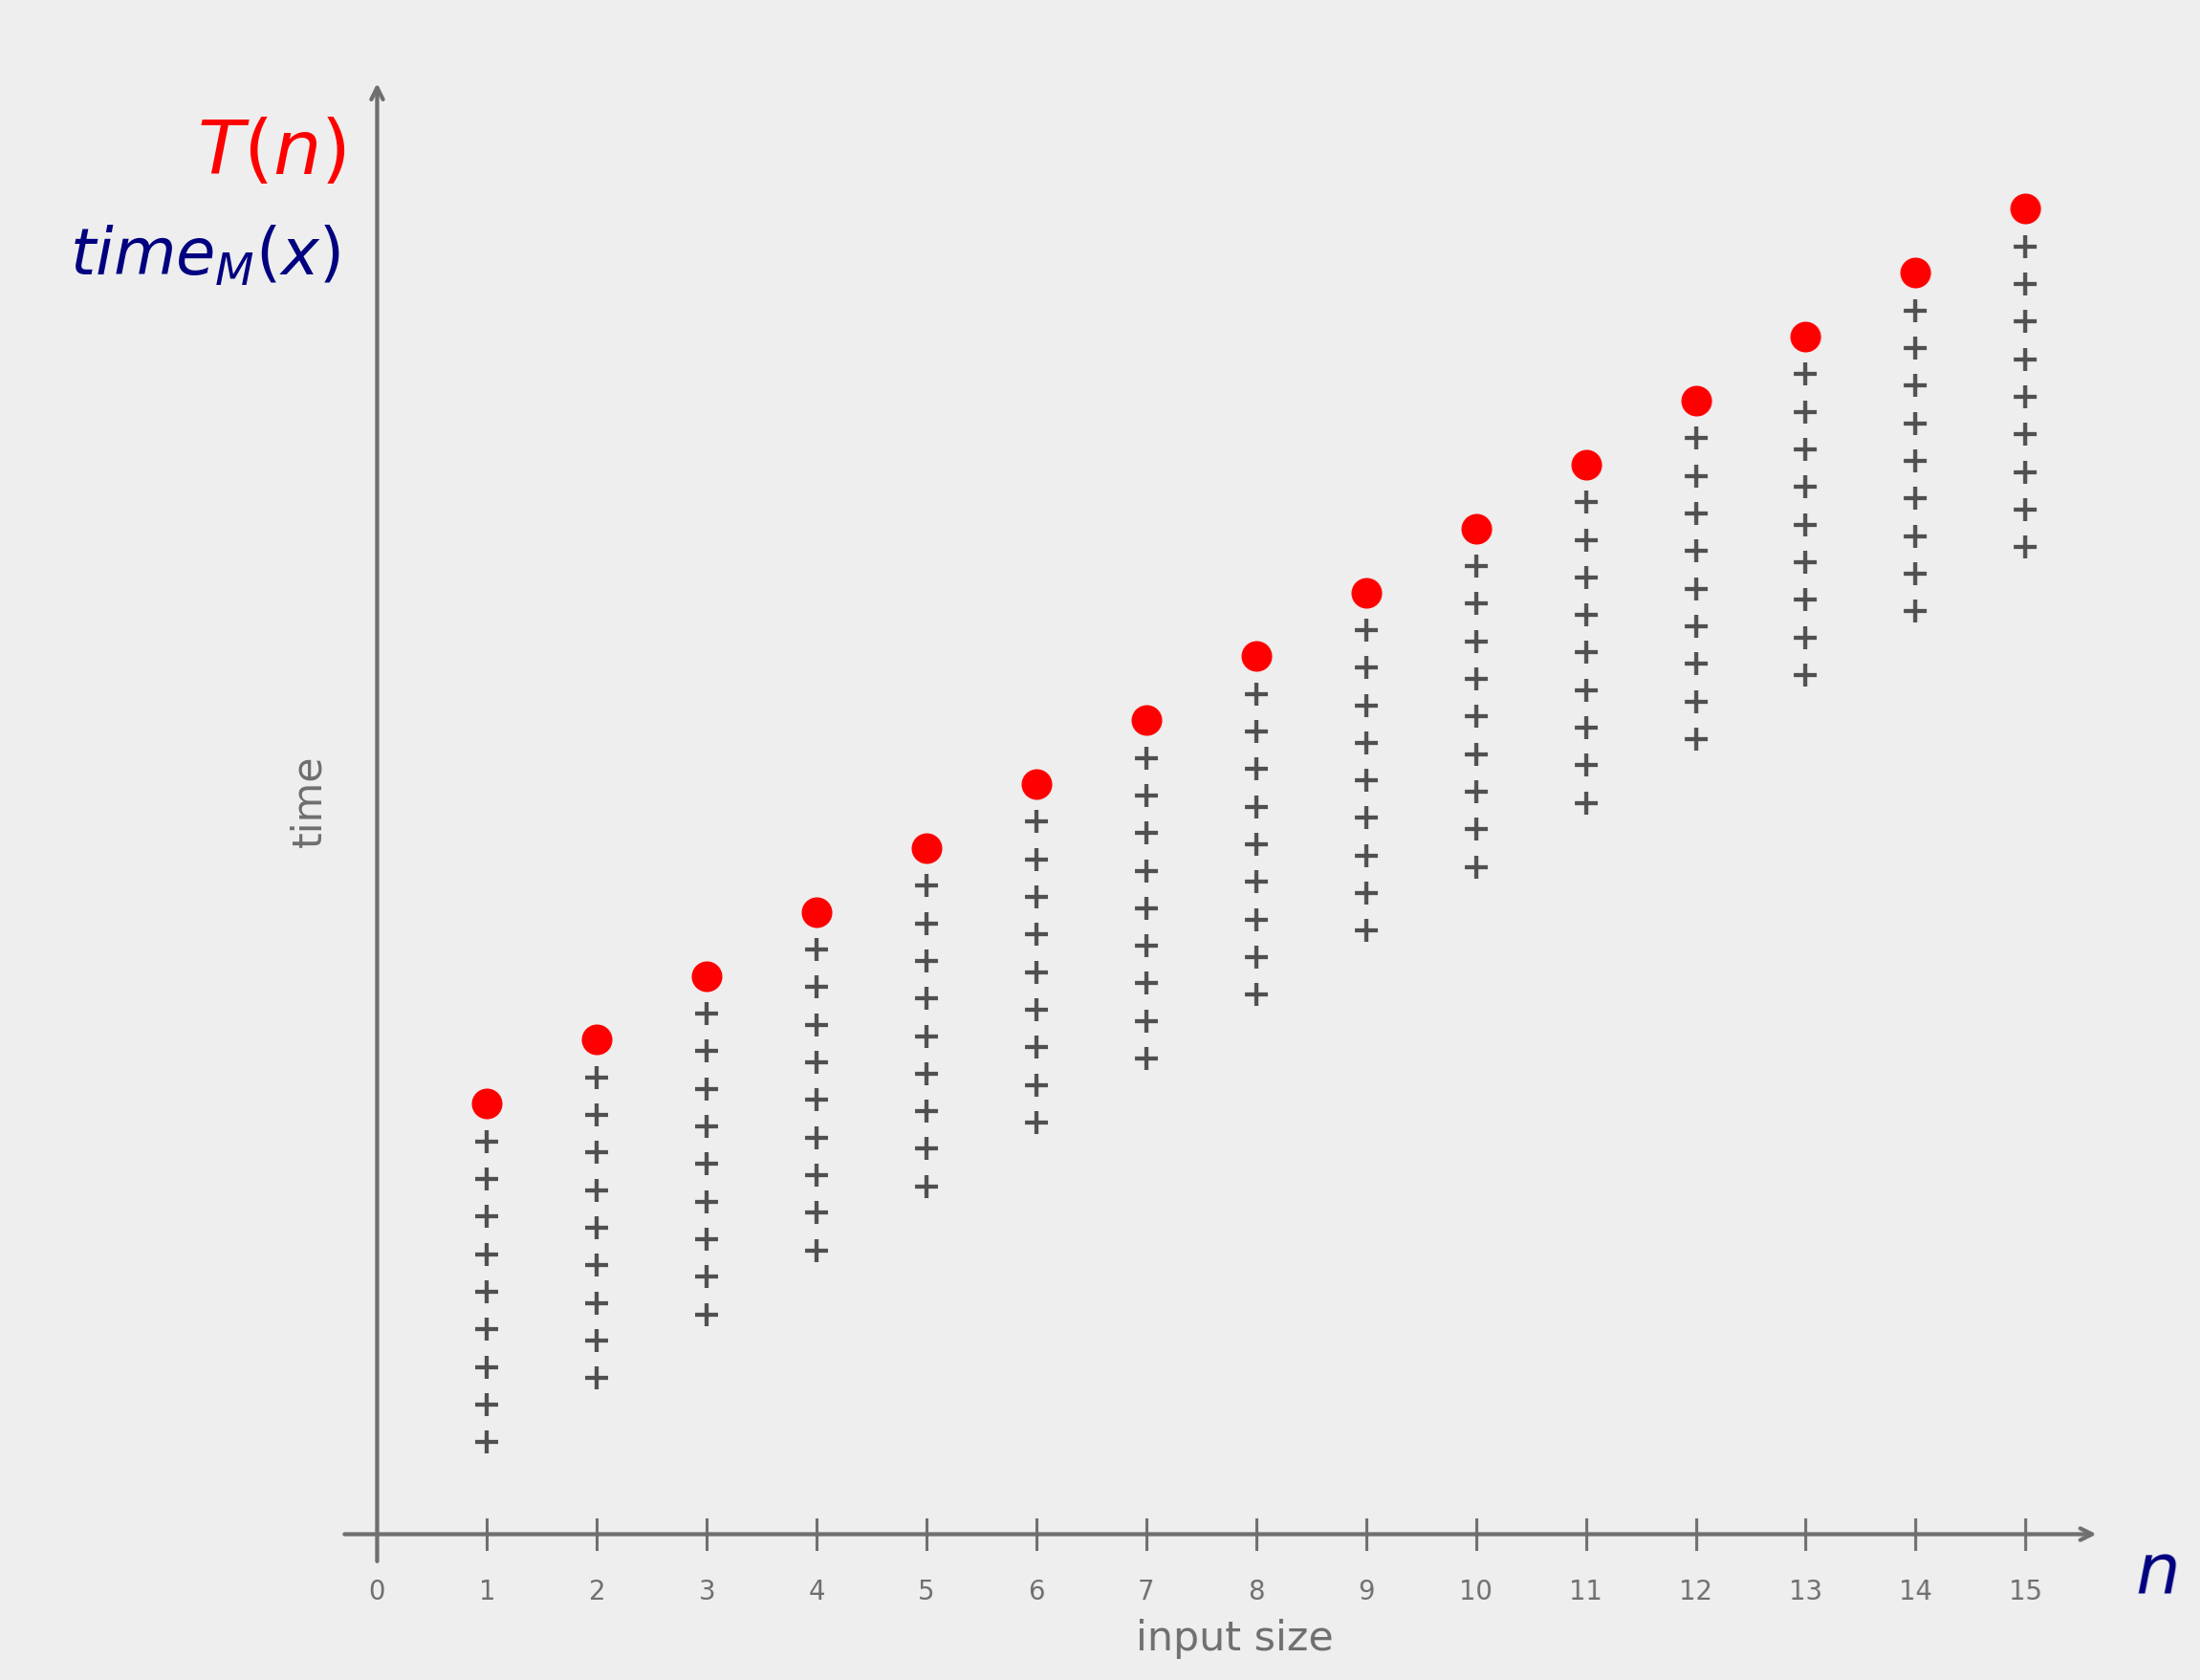
\includegraphics[width=0.78\textwidth]{Figures/worst_case.png}
    \caption{Časová složitost v nejhorším případě podle \cite{sawa_ti_03}}
    \label{fig:worst_case_complexity}
\end{figure}

Obrázek \ref{fig:worst_case_complexity} ukazuje, že pro vstupy stejné velikosti nemusí algoritmus vždy vykonat stejný počet operací. Časová složitost v nejhorším případě proto sleduje maximální hodnotu těchto nákladů a poskytuje tak bezpečný odhad horní meze časové náročnosti algoritmu.

Vedle časové složitosti v nejhorším případě má smysl zkoumat také časovou složitost v průměrném případě. V tomto případě není funkce \(T(n)\) určena maximální hodnotou přes všechny vstupy dané velikosti, ale aritmetickým průměrem odpovídajících nákladů. Určení průměrného případu však bývá zpravidla obtížnější než určení nejhoršího případu, protože vyžaduje přesnější představu o množině vstupů a jejich rozdělení. Ve většině případů se proto při analýze algoritmů častěji vychází právě z nejhoršího případu \cite{sawa_ti_03}.

Pro názornost je na obrázku \ref{fig:average_case_complexity} znázorněna časová složitost v průměrném případě. Na rozdíl od nejhoršího případu zde funkce \(T(n)\) nepředstavuje horní obálku všech hodnot, ale jejich průměrné chování pro vstupy stejné velikosti.

\begin{figure}[H]
    \centering
    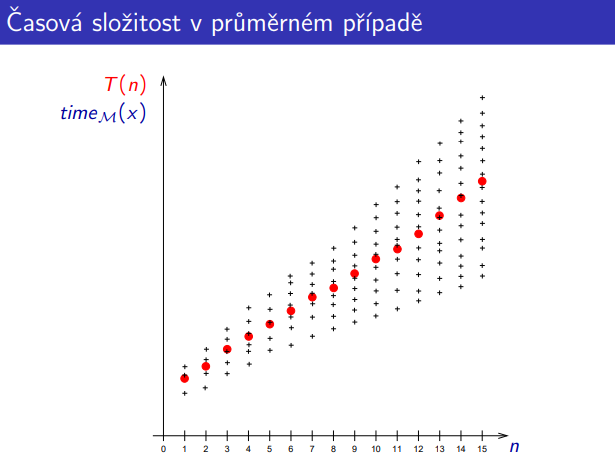
\includegraphics[width=0.78\textwidth]{Figures/average_case.png}
    \caption{Časová složitost v průměrném případě podle \cite{sawa_ti_03}}
    \label{fig:average_case_complexity}
\end{figure}

Časová složitost v nejhorším a průměrném případě se často příliš neliší, i když v některých situacích může být rozdíl významný. Zároveň se uvádí, že zkoumání složitosti v nejlepším případě obvykle nemá příliš velký praktický význam \cite{sawa_ti_03}.

\newpage

\subsection{Asymptotická notace a třídy růstu funkcí}
Přesné vyjádření časové složitosti bývá často komplikované a silně závisí na zvoleném výpočetním modelu i na detailech implementace. Ve většině případů navíc není nutné znát přesný počet instrukcí, ale stačí odhadnout, jak rychle tento počet roste se zvětšující se velikostí vstupu. Právě z tohoto důvodu se zavádí asymptotická notace, která zanedbává méně podstatné detaily a umožňuje soustředit se na dominantní složku růstu sledované funkce \cite{sawa_ti_03}.

V rámci asymptotické notace se nejčastěji používají symboly \(O\), \(\Omega\) a \(\Theta\). Zápis \(O(g(n))\) vyjadřuje horní asymptotickou mez růstu funkce, tedy skutečnost, že sledovaná funkce neroste rychleji než funkce \(g(n)\) až na konstantní násobek. Naopak \(\Omega(g(n))\) vyjadřuje dolní asymptotickou mez a \(\Theta(g(n))\) charakterizuje situaci, kdy funkce roste stejnou rychlostí jako \(g(n)\) z hlediska horní i dolní meze současně. Kromě těchto symbolů se používají také \(o(g(n))\) a \(\omega(g(n))\), které popisují přísně pomalejší, respektive přísně rychlejší růst \cite{sawa_ti_03}.

Big-O notace popisuje asymptotické chování funkcí a umožňuje při analýze algoritmů zanedbat konstanty i pomaleji rostoucí členy \cite{mit_big_o}. Mezi běžné třídy patří například \(O(1)\), \(O(\log n)\), \(O(n)\), \(O(n^2)\), polynomiální růst a exponenciální růst, přičemž exponenciální funkce rostou výrazně rychleji než funkce polynomiální \cite{mit_big_o}.

Na základě asymptotického chování lze algoritmy rozdělovat do několika základních tříd. Za logaritmické se považují algoritmy se složitostí \(\Theta(\log n)\), za lineární algoritmy se složitostí \(\Theta(n)\), za kvadratické se považují algoritmy se složitostí \(\Theta(n^2)\) a podobně. Významnou skupinu tvoří také polynomiální algoritmy, tedy algoritmy, jejichž časová složitost je shora omezena nějakým polynomem. Naopak exponenciální nebo faktoriální složitosti obvykle vedou k tomu, že algoritmus je použitelný pouze pro velmi malé vstupy \cite{sawa_ti_03,mit_big_o}.

Praktický význam rozdílné rychlosti růstu funkcí ukazuje tabulka \ref{tab:growth_rate_functions}. Ta vychází z předpokladu, že algoritmus zpracovává vstup velikosti \(n\), provede \(T(n)\) operací a provedení jedné operace trvá \(1\,\mu s\). Je z ní patrné, že rozdíly mezi jednotlivými třídami složitosti se s rostoucí velikostí vstupu velmi rychle zvětšují \cite{sawa_ti_03}.

\begin{table}[H]
\centering
\caption{Příklad růstu doby výpočtu pro vybrané třídy časové složitosti podle \cite{sawa_ti_03}}
\label{tab:growth_rate_functions}

\setlength{\tabcolsep}{3pt}
\renewcommand{\arraystretch}{1.15}
\scriptsize

\resizebox{\textwidth}{!}{%
\begin{tabular}{|c|c|c|c|c|c|c|c|c|}
\hline
    \(T(n)\) / \(n\) & 20 & 40 & 60 & 80 & 100 & 200 & 500 & 1000 \\ \hline
    \(n\) & 20 \(\mu s\) & 40 \(\mu s\) & 60 \(\mu s\) & 80 \(\mu s\) & 0.1 ms & 0.2 ms & 0.5 ms & 1 ms \\ \hline
    \(n \log n\) & 86 \(\mu s\) & 0.213 ms & 0.354 ms & 0.506 ms & 0.664 ms & 1.528 ms & 4.48 ms & 9.96 ms \\ \hline
    \(n^2\) & 0.4 ms & 1.6 ms & 3.6 ms & 6.4 ms & 10 ms & 40 ms & 0.25 s & 1 s \\ \hline
    \(n^3\) & 8 ms & 64 ms & 0.216 s & 0.512 s & 1 s & 8 s & 125 s & 16.7 min. \\ \hline
    \(n^4\) & 0.16 s & 2.56 s & 12.96 s & 42 s & 100 s & 26.6 min. & 17.36 hod. & 11.57 dní \\ \hline
    \(2^n\) & 1.05 s & 12.75 dní & 36560 let & \(38.3 \cdot 10^9\) let & \(40.1 \cdot 10^{15}\) let & \(50 \cdot 10^{45}\) let & \(10.4 \cdot 10^{136}\) let & -- \\ \hline
    \(n!\) & 77147 let & \(2.59 \cdot 10^{34}\) let & \(2.64 \cdot 10^{68}\) let & \(2.27 \cdot 10^{105}\) let & \(2.96 \cdot 10^{144}\) let & -- & -- & -- \\ \hline
\end{tabular}%
}
\end{table}

Z tabulky \ref{tab:growth_rate_functions} je patrné, že i relativně malé rozdíly v asymptotické třídě mohou mít při větších vstupech zásadní dopad na skutečnou dobu výpočtu. Zatímco lineární nebo logaritmické algoritmy zůstávají použitelné i pro velké vstupy, algoritmy s exponenciální nebo faktoriální složitostí se stávají prakticky neproveditelnými velmi rychle \cite{sawa_ti_03,mit_big_o}.

\subsection{Praktický význam časové složitosti}
Při interpretaci asymptotické notace je však nutné mít na paměti i její omezení. Asymptotické odhady vypovídají pouze o tom, jak roste náročnost s rostoucí velikostí vstupu, ale neříkají nic o skutečné době běhu na konkrétním počítači. V notaci mohou být navíc skryty velké konstanty, takže algoritmus s asymptoticky lepší složitostí nemusí být v praxi rychlejší pro malé nebo středně velké vstupy \cite{sawa_ti_03}.

Tuto skutečnost lze ilustrovat také na třídicích algoritmech. Například quicksort má v nejhorším případě složitost \(\Theta(n^2)\), zatímco heapsort \(\Theta(n \log n)\), ale přesto bývá quicksort v praxi často velmi rychlý. Z toho vyplývá, že časová složitost je sice velmi důležitým nástrojem pro porovnávání algoritmů, ale při hodnocení konkrétního řešení je třeba zohlednit i další okolnosti.

Z praktického hlediska bývají za efektivní považovány především algoritmy s polynomiální časovou složitostí. Ani zde však nelze formulovat zcela absolutní závěry, protože například algoritmus se složitostí \(\Theta(n^{100})\) je sice formálně polynomiální, avšak z praktického hlediska obtížně použitelný. Naopak některé algoritmy s horší teoretickou složitostí mohou být pro malé vstupy nebo specifické úlohy stále využitelné \cite{sawa_ti_03,mit_big_o}.

Pro potřeby této práce je důležité, že klasická časová složitost obvykle hodnotí náklady jednotlivých výpočtů nebo jednotlivých operací vzhledem k velikosti vstupu. U některých datových struktur a algoritmů však může být vhodnější sledovat celkové náklady delší posloupnosti operací. Právě tímto pohledem se zabývá amortizovaná analýza, která je tématem následující části kapitoly \cite{tarjan1985amortized,kozen_amortized}.



\section{Amortizovaná složitost a její význam}
V této podkapitole je nejprve vymezen pojem amortizované složitosti a vysvětlen základní princip tohoto způsobu analýzy. Následně je pozornost věnována významu amortizované analýzy při hodnocení algoritmů a datových struktur. V závěru této podkapitoly je amortizovaná analýza srovnána s dalšími přístupy používanými při posuzování náročnosti algoritmů.

\subsection{Vymezení amortizované složitosti}
Amortizovaná složitost představuje způsob hodnocení algoritmů a datových struktur, při němž se nesleduje pouze cena jedné izolované operace, ale celkové náklady delší posloupnosti operací. Tento přístup vychází z toho, že jednotlivé operace v posloupnosti nemusí mít stejnou cenu. Některé mohou být velmi levné, jiné naopak výrazně dražší, a proto by samostatné hodnocení jedné operace mohlo vést ke zkreslenému pohledu na skutečné chování algoritmu \cite{tarjan1985amortized,kozen_amortized}.

Amortizovaná analýza představuje analýzu posloupnosti operací v nejhorším případě, jejímž cílem je získat těsnější odhad celkových nebo průměrných nákladů na jednu operaci, než kdyby byla každá operace analyzována samostatně \cite{kozen_amortized}. Z toho vyplývá, že dražší operace nejsou posuzovány izolovaně, ale v souvislosti s ostatními operacemi v posloupnosti. Jejich vysoká cena se tak rozkládá mezi více levnějších operací, takže dlouhodobé chování algoritmu může být z hlediska jedné operace příznivější.

\subsection{Význam amortizované analýzy}
Význam amortizované analýzy spočívá především v tom, že poskytuje realističtější pohled na chování algoritmů a datových struktur v situacích, kdy se náklady jednotlivých operací výrazně liší. Amortizace je chápána jako technika „zprůměrování v čase“ a amortizovaná doba běhu představuje realistickou a zároveň robustní míru složitosti \cite{tarjan1985amortized}. Tento přístup je užitečný zejména tam, kde se vyskytují občasné drahé operace, které jsou však v delší posloupnosti kompenzovány velkým množstvím operací levných.

Amortizovaná analýza je důležitá také proto, že se nespoléhá na pravděpodobnostní předpoklady o rozdělení vstupů. Oproti průměrnému případu není založena na odhadu, jak často se určitý typ vstupu vyskytne. Hodnocení je prováděno nad posloupností operací v nejhorším případě a může vést k přesnějším odhadům, než kdyby byly jednotlivé operace posuzovány odděleně \cite{kozen_amortized}. Tato vlastnost představuje výhodu zejména u datových struktur, jejichž stav se v čase mění a kde jsou jednotlivé operace vzájemně závislé.

Z hlediska návrhu algoritmů a datových struktur je amortizovaná analýza přínosná i tím, že umožňuje lépe vysvětlit, proč mohou být některá řešení v praxi efektivní, i když obsahují občasné nákladné kroky. Pokud je totiž celková cena dlouhé posloupnosti operací příznivá, může být daná datová struktura nebo algoritmus vhodným řešením i přesto, že jednotlivé operace nemají vždy malou cenu nejhoršího případu.

\subsection{Srovnání s ostatními přístupy}
Amortizovanou analýzu je vhodné odlišit od dalších běžných přístupů používaných při hodnocení algoritmů. Nejhorší případ sleduje maximální cenu jedné operace nebo jednoho běhu algoritmu. Průměrný případ naopak vyjadřuje očekávanou cenu vzhledem k určitému rozdělení vstupů. Amortizovaná analýza se od obou těchto přístupů liší tím, že hodnotí celou posloupnost operací a z ní odvozuje náklady připadající na jednu operaci \cite{kozen_amortized,tarjan1985amortized}.

Je důležité zdůraznit, že amortizovaná složitost není totéž co složitost průměrná. Průměrná složitost vychází z pravděpodobnostního modelu vstupů, zatímco amortizovaná analýza žádné takové předpoklady nepotřebuje. Nejedná se tedy o statistický průměr přes různé vstupy, ale o rozložení nákladů v rámci posloupnosti operací. Právě v tom spočívá její významná odlišnost i její praktická síla \cite{kozen_amortized}.

Pro lepší přehlednost shrnuje tabulka \ref{tab:comparison_complexity_approaches} základní rozdíly mezi třemi běžnými přístupy k hodnocení náročnosti algoritmů.

\begin{table}[H]
\centering
\caption{Srovnání vybraných přístupů k hodnocení složitosti}
\label{tab:comparison_complexity_approaches}
\begin{tabular}{|p{3.2cm}|p{3.9cm}|p{5.2cm}|}
\hline
    \textbf{Přístup} & \textbf{Co sleduje} & \textbf{Charakteristika} \\ \hline
    Nejhorší případ & Maximální cenu jedné operace nebo jednoho běhu & Poskytuje bezpečnou horní mez, ale může být příliš pesimistický. \\ \hline
    Průměrný případ & Průměrnou cenu vzhledem k rozdělení vstupů & Závisí na předpokladech o vstupních datech a jejich pravděpodobnosti. \\ \hline
    Amortizovaná analýza & Celkové náklady posloupnosti operací & Rozkládá cenu dražších operací mezi větší počet levnějších operací a nevyžaduje pravděpodobnostní model vstupů. \\ \hline
\end{tabular}
\end{table}

Ze srovnání vyplývá, že amortizovaná analýza zaujímá mezi ostatními přístupy zvláštní postavení. Zachovává výhodu pohledu nejhoršího případu v tom, že neposkytuje pouze optimistický odhad založený na pravděpodobnosti, ale zároveň dovoluje přesněji zachytit skutečné dlouhodobé chování algoritmu. Díky tomu je vhodná pro analýzu datových struktur, u nichž se stav postupně mění a kde některé operace ovlivňují cenu operací následujících \cite{tarjan1985amortized}.

Na základní vymezení pojmu amortizované složitosti navazují další části této kapitoly, které se podrobněji věnují jednotlivým metodám amortizované analýzy a jejich praktickému použití.



\section{Metody amortizované analýzy}
V této podkapitole jsou stručně popsány základní metody amortizované analýzy, které se využívají při hodnocení algoritmů a datových struktur. Pozornost je věnována agregované metodě, účetní metodě a potenciálové metodě. Na závěr jsou shrnuty jejich základní vlastnosti a vzájemné rozdíly.

\newpage

\subsection{Agregovaná metoda}
Agregovaná metoda představuje nejjednodušší způsob amortizované analýzy. Jejím základním principem je sledování celkových nákladů celé posloupnosti operací a následné odvození průměrných nákladů připadajících na jednu operaci. Místo samostatného hodnocení jednotlivých operací se tedy analyzuje celkový součet jejich cen. Pokud lze ukázat, že posloupnost \(m\) operací má celkovou cenu \(O(m)\), je možné usoudit, že amortizovaná cena jedné operace je konstantní \cite{kozen_amortized,cmu_amortized}.

Výhodou agregované metody je její jednoduchost a přehlednost. Hodí se zejména v situacích, kdy lze celkové náklady celé posloupnosti vyjádřit přímo a bez zavádění dalších pomocných veličin. Naopak u složitějších datových struktur bývá tato metoda méně flexibilní \cite{cmu_amortized}.

\subsection{Účetní metoda}
Účetní metoda, označovaná také jako bankéřská metoda, vychází z představy, že jednotlivým operacím lze přiřadit určitou účtovanou cenu, která se může lišit od jejich skutečné ceny. Levnějším operacím je přiřazena vyšší cena, než jakou ve skutečnosti mají, a vzniklý přebytek se uchovává jako rezerva pro budoucí dražší operace. Díky tomu je možné rozložit cenu nákladnějších kroků mezi větší počet kroků, které jsou levnější \cite{kozen_amortized,cmu_amortized}.

U této metody je důležité, aby nahromaděná rezerva v průběhu celé posloupnosti operací nikdy neklesla pod nulu. Účetní metoda tak názorně ukazuje, že některé operace si mohou vytvářet rezervu pro budoucí nákladnější kroky \cite{cmu_amortized}.

\subsection{Potenciálová metoda}
Potenciálová metoda pracuje s potenciálovou funkcí, která vyjadřuje stav datové struktury a určitou rezervu nahromaděnou v systému. Amortizovaná cena operace je zde určena jako součet její skutečné ceny a změny potenciálu mezi stavem před operací a po ní \cite{kozen_amortized,cmu_amortized}. Vzhledem k její obecnosti a významu bude tato metoda podrobněji vysvětlena v následující části kapitoly.

\subsection{Vztah mezi jednotlivými metodami}
Všechny tři metody sledují stejný cíl, tedy získání vhodného odhadu nákladů dlouhé posloupnosti operací. Liší se však způsobem, jakým k tomuto cíli docházejí. Agregovaná metoda pracuje s celkovým součtem nákladů celé posloupnosti, účetní metoda zavádí účtované ceny a rezervy a potenciálová metoda využívá potenciálovou funkci popisující stav datové struktury \cite{kozen_amortized,cmu_amortized,tarjan1985amortized}.

Pro lepší přehlednost shrnuje tabulka \ref{tab:methods_amortized_analysis} základní vlastnosti těchto metod.

\begin{table}[H]
\centering
\caption{Základní metody amortizované analýzy}
\label{tab:methods_amortized_analysis}
\begin{tabular}{|p{3.2cm}|p{4.2cm}|p{4.8cm}|}
\hline
    \textbf{Metoda} & \textbf{Základní princip} & \textbf{Charakteristika} \\ \hline
    Agregovaná metoda & Sleduje celkovou cenu celé posloupnosti operací & Nejjednodušší přístup, vhodný pro případy, kdy lze celkové náklady snadno vyjádřit. \\ \hline
    Účetní metoda & Přiřazuje operacím účtované ceny a vytváří rezervu pro dražší operace & Umožňuje rozložit cenu nákladných operací mezi levnější operace v posloupnosti. \\ \hline
    Potenciálová metoda & Pracuje s potenciálovou funkcí vyjadřující stav datové struktury & Obecný a formální přístup, vhodný pro přesnější analýzu složitějších struktur. \\ \hline
\end{tabular}
\end{table}

Z uvedeného srovnání vyplývá, že jednotlivé metody nejsou ve vzájemném rozporu, ale spíše představují různé pohledy na tentýž problém. Zatímco agregovaná metoda bývá nejjednodušší na použití, potenciálová metoda nabízí největší obecnost a formální sílu. Právě proto je v další části této kapitoly podrobněji rozebrána.



\section{Potenciálová metoda}
V této části je podrobněji vysvětlena potenciálová metoda. Pozornost je věnována jejímu principu, způsobu vyjádření amortizované ceny operace a významu potenciálové funkce při hodnocení změn stavu datové struktury. V závěru této části jsou shrnuty hlavní výhody potenciálové metody ve srovnání s ostatními přístupy.

\subsection{Princip potenciálové metody}
Potenciálová metoda patří mezi základní metody amortizované analýzy a představuje obecný způsob, jak vyjádřit vztah mezi skutečnými náklady jednotlivých operací a jejich dlouhodobým chováním v celé posloupnosti operací. Vychází z předpokladu, že aktuální stav datové struktury může nést určitou rezervu pro budoucí nákladnější operace. Tato rezerva je popsána pomocí potenciálové funkce \cite{tarjan1985amortized,kozen_amortized,cmu_amortized}.

Potenciálová metoda proto nesleduje pouze skutečnou cenu právě prováděné operace, ale také to, jak se po jejím provedení změní stav celé datové struktury. Díky tomu umožňuje přesněji zachytit celkové chování delších posloupností operací než izolované hodnocení jednotlivých kroků. Ve srovnání s agregovanou a účetní metodou je abstraktnější, ale zároveň poskytuje obecný a formální nástroj, který je vhodný i pro složitější důkazy amortizované složitosti \cite{cmu_amortized}.

\subsection{Potenciálová funkce a amortizovaná cena operace}
Klíčovým pojmem této metody je potenciálová funkce, obvykle značená \(\Phi\). Tato funkce přiřazuje každému stavu datové struktury určitou číselnou hodnotu, která vyjadřuje velikost nahromaděné rezervy v daném stavu. Potenciál tedy nepředstavuje skutečný čas ani skutečný počet instrukcí, ale pomocnou veličinu, která umožňuje lépe vyjádřit rozložení nákladů mezi jednotlivé operace \cite{tarjan1985amortized,kozen_amortized}.

Je-li skutečná cena \(i\)-té operace označena jako \(c_i\), stav datové struktury před provedením operace jako \(D_{i-1}\) a stav po jejím provedení jako \(D_i\), pak amortizovaná cena této operace může být zapsána ve tvaru \[\hat{c}_i = c_i + \Phi(D_i) - \Phi(D_{i-1}).\]

Tento vztah vyjadřuje, že amortizovaná cena operace se skládá ze skutečné ceny operace a změny potenciálu mezi stavem před operací a po ní. Pokud se potenciál po operaci zvětší, znamená to, že se vytváří rezerva pro budoucí operace. Pokud se naopak potenciál zmenší, dochází k využití dříve nahromaděné rezervy \cite{tarjan1985amortized,cmu_amortized}.

Důležitou vlastností potenciálové funkce je, že by měla být zvolena tak, aby její hodnoty byly nezáporné, případně aby počáteční stav neměl záporný potenciál. Díky tomu lze ukázat, že součet amortizovaných cen celé posloupnosti poskytuje horní odhad součtu jejich skutečných cen. Potenciálová metoda tak umožňuje dokázat, že i když některé operace mohou být drahé, jejich cena je v delší posloupnosti vyvážena operacemi jinými \cite{kozen_amortized,cmu_amortized}.

Z praktického hlediska je při volbě potenciálové funkce důležité, aby odpovídala vlastnostem konkrétní datové struktury a správně vystihovala, jakým způsobem systém vytváří a spotřebovává rezervu. Právě volba vhodné potenciálové funkce bývá při důkazu amortizované složitosti jedním z nejdůležitějších kroků.

\subsection{Význam a využití potenciálové metody}
Význam potenciálové metody spočívá především v její obecnosti a formální síle. Ve srovnání s ostatními metodami amortizované analýzy umožňuje velmi přesně popsat změny stavu datové struktury a jejich vliv na cenu budoucích operací. Díky tomu je vhodná i pro analýzu složitějších struktur, u nichž nestačí pouze sledovat celkový součet nákladů nebo intuitivně rozdělovat rezervu mezi jednotlivé operace \cite{tarjan1985amortized,cmu_amortized}.

Potenciálová metoda je užitečná zejména v situacích, kdy se stav datové struktury v čase výrazně mění a kdy některé operace přímo ovlivňují náročnost operací následujících. V takovém případě poskytuje přirozený způsob, jak vyjádřit, že nákladnější operace nejsou izolovaným jevem, ale souvisejí s vývojem celého systému. To je také důvod, proč je tato metoda často považována za nejuniverzálnější z běžně používaných metod amortizované analýzy.

Z hlediska této práce je potenciálová metoda důležitá i proto, že umožňuje názorně propojit teoretický princip amortizované analýzy s konkrétním chováním algoritmů a datových struktur. Pomocí potenciálu lze sledovat, jak se v jednotlivých stavech vytváří nebo spotřebovává rezerva, a tím lépe vysvětlit, proč nelze cenu některých algoritmů hodnotit pouze podle jedné samostatné operace. Právě tato vlastnost činí potenciálovou metodu vhodnou nejen pro teoretickou analýzu, ale i pro výukové a vizualizační účely.



\section{Vybrané algoritmy vhodné pro amortizovanou analýzu}
V této podkapitole jsou stručně představeny algoritmy, u nichž je amortizovaná analýza vhodným nástrojem pro hodnocení jejich chování. Nejprve jsou uvedeny některé příklady algoritmů, u nichž se tento přístup běžně využívá. Následně jsou zmíněny algoritmy vybrané do praktické části této práce a na závěr jsou přehledně shrnuty.

\subsection{Algoritmy vhodné pro amortizovanou analýzu}
Amortizovaná analýza se uplatňuje zejména u algoritmů, u nichž se jednotlivé operace mohou lišit svou skutečnou cenou, avšak při delší posloupnosti operací vykazuje celý systém příznivější chování. Tento přístup je vhodný především tehdy, když se vyskytují občasné nákladnější operace, jejichž cenu lze rozložit mezi větší počet operací levnějších. Typickou situací je stav, kdy se mění datová struktura a některé operace ovlivňují náročnost operací následujících.

Mezi často uváděné příklady algoritmů vhodných pro amortizovanou analýzu patří například:
\begin{itemize}
    \item Multipop na zásobníku,
    \item Fronta využívající dva zásobníky,
    \item Splay strom,
    \item Dynamické pole s občasným rozšířením kapacity,
    \item Binární čítač,
    \item některé operace nad disjoint-set strukturami.
\end{itemize}

Tyto algoritmy mají společné to, že jednotlivé operace nemusí mít vždy stejnou cenu, ale v delší posloupnosti operací lze jejich chování pomocí amortizované analýzy popsat přesněji, než kdyby bylo hodnoceno pouze izolovaně po jednotlivých krocích.

\subsection{Algoritmy vybrané do praktické části práce}
Do praktické části této bakalářské práce byly vybrány tři algoritmy: Multipop na zásobníku, fronta využívající dva zásobníky a Splay strom. Tyto algoritmy byly zvoleny tak, aby společně tvořily trojici příkladů různé obtížnosti a zároveň umožňovaly názorně ukázat různé projevy amortizované složitosti.

\newpage

\subsection{Přehled vybraných algoritmů}
Pro lepší přehlednost shrnuje tabulka \ref{tab:selected_algorithms_amortized} algoritmy vybrané do praktické části práce.

\begin{table}[H]
\centering
\caption{Vybrané algoritmy vhodné pro amortizovanou analýzu}
\label{tab:selected_algorithms_amortized}
\begin{tabular}{|p{4cm}|p{2.3cm}|p{6cm}|}
\hline
    \textbf{Algoritmus} & \textbf{Obtížnost} & \textbf{Stručná charakteristika} \\ \hline
    Multipop na zásobníku & jednoduchá & Jednoduchý příklad ukazující, že jedna dražší operace může být v delší posloupnosti nákladově vyvážena. \\ \hline
    Fronta využívající dva zásobníky & střední & Příklad rozložení nákladů mezi operace enqueue a dequeue při implementaci fronty pomocí dvou zásobníků. \\ \hline
    Splay strom & vyšší & Pokročilejší datová struktura, u níž se amortizovaná analýza používá pro popis chování po sérii přístupových operací. \\ \hline
\end{tabular}
\end{table}

Z uvedeného přehledu je patrné, že vybrané algoritmy pokrývají různé úrovně obtížnosti i různé způsoby projevu amortizované složitosti. Právě proto tvoří vhodný základ pro praktickou část této práce, v níž budou dále využity pro vytvoření názorné výukové vizualizace.
\chapter{Návrh komponenty výukového serveru}
Třetí kapitola se primárně věnuje návrhu komponenty výukového serveru zaměřené na problematiku amortizované složitosti. Nejprve popisuje cíl a roli navrhované komponenty v rámci výukového serveru a vysvětluje její přínos pro výuku této oblasti. Následně shrnuje hlavní požadavky, které byly na komponentu kladeny, a objasňuje výběr algoritmů zařazených do praktické části práce. Další část kapitoly se zaměřuje na návrh funkcionality komponenty, zejména na způsoby zadávání vstupů, zobrazení průběhu algoritmů a prezentaci hodnot důležitých pro pochopení amortizované analýzy. Na konci kapitoly je pozornost věnována také návrhu uživatelského rozhraní, celkové struktury komponenty a možného rozšíření. 



\section{Cíl a role navrhované komponenty}
V této části je nejprve vymezeno zařazení navrhované komponenty v rámci výukového serveru. Následně je pozornost věnována hlavnímu účelu komponenty a její roli při zprostředkování problematiky amortizované složitosti studentům. V závěru této části je shrnut její přínos pro výuku a pro názornější pochopení sledované problematiky.

\newpage

\subsection{Zařazení komponenty do výukového serveru}
Vytvořená komponenta vzniká jako součást výukového serveru určeného pro předměty TI. Tento výukový server má mít podobu sady dynamických webových stránek, jejichž hlavním cílem je umožnit budoucím studentům lépe pochopit principy různých typů úloh a problémů prostřednictvím názorných a interaktivních ukázek. Na rozdíl od běžných statických výukových materiálů, které obvykle pracují pouze s pevně daným počtem příkladů, má takové řešení umožnit generovat libovolný počet ukázkových příkladů vybraných algoritmů na základě vstupů od uživatele a sledovat jejich průběh v různých situacích.

Navrhovaná komponenta je v rámci tohoto serveru zaměřena na oblast amortizované složitosti. Jejím úkolem je rozšířit výukový server o část, která studentům umožní lépe pochopit principy tohoto typu analýzy na konkrétních algoritmech a datových strukturách. Komponenta se tedy nesnaží představit samostatný izolovaný nástroj, ale stává se součástí výuky v TI a zapadá do širšího konceptu interaktivní podpory studia teoretické informatiky.

\subsection{Hlavní účel komponenty}
Hlavním účelem této navržené komponenty je vytvořit prostředek pro pochopení počítání složitosti vybraných algoritmů s využitím amortizované analýzy, která byla podrobně popsána v předchozí kapitole. Komponenta má budoucím studentům poskytnout vizualizaci toho, jak se algoritmus chová při zpracování vstupu, jak se mění stav dané datové struktury a jak probíhá vývoj hodnot v jednotlivých krocích, které jsou důležité pro amortizovanou analýzu. Důraz je kladen především na to, aby uživatel viděl podrobný průběh algoritmu v každém kroku, nikoli pouze konečný výsledek výpočtu.

Účelem komponenty tedy není pouze umožnit spuštění algoritmu, ale především podpořit hlubší pochopení celého principu, proč se amortizovaná složitost hodnotí v rámci delší posloupnosti operací. Komponenta má propojit teoretický výklad s názornou ukázkou chování algoritmu a nabídnout studentovi možnost sledovat souvislosti mezi jednotlivými operacemi a jejich dlouhodobým dopadem.

\newpage

\subsection{Přínos komponenty pro výuku amortizované složitosti}
Celá problematika amortizované složitosti bývá pro studenty často obtížně pochopitelná, protože její správné pochopení vyžaduje sledování souvislostí mezi více operacemi, změn stavů vizualizovaných datových struktur a vývoje hodnot, které se při amortizované analýze používají. Klasické výklady v teoretické formě pomocí prezentací, skript nebo několika málo statických ukázek nemusí vždy stačit k tomu, aby si studenti vytvořili dostatečně jasnou představu o tom, proč se některé operace mohou jevit jako nákladné oproti ostatním a proč je přesto možné celkové chování algoritmu hodnotit příznivěji.

Důležitý přínos této komponenty spočívá především v propojení teoretického výkladu s názornou praktickou ukázkou. Student může při práci s komponentou aktivně sledovat průběh algoritmů, pozorovat změny stavů datových struktur a lépe chápat vztah mezi jednotlivými operacemi a jejich dlouhodobým chováním. Komponenta tak může přispět k názornější a srozumitelnější výuce amortizované složitosti v rámci předmětů TI.



\section{Požadavky na komponentu}
Tato část se zaměřuje na hlavní požadavky, které byly na navrhovanou komponentu kladeny. Nejprve jsou shrnuty funkční požadavky související s chováním a možnostmi komponenty. Následně jsou popsány požadavky na uživatelskou interakci a na způsob, jakým má uživatel s komponentou pracovat. Závěr této části je věnován požadavkům na názornost a výukovou hodnotu navrhovaného řešení.

\subsection{Funkční požadavky}
Při návrhu celé komponenty bylo potřeba vycházet z požadavků, které byly stanoveny v zadání bakalářské práce. Základním funkčním požadavkem bylo vytvořit dynamické webové stránky, které umožní vhodným způsobem zobrazit simulaci běhu alespoň tří různých algoritmů, u nichž je vhodné analyzovat složitost pomocí amortizované analýzy. Komponenta tak měla uživateli umožnit nejen samotné spuštění algoritmu, ale také sledování jeho jednotlivých kroků v průběhu zpracování zadaného vstupu.

Dalším důležitým požadavkem bylo umožnit uživateli zadávat vstupy více různými způsoby. Návrh u každého algoritmu proto musel počítat s možností ručního zadávání vstupů, s generováním náhodných vstupů podle zvolených parametrů, s prací s různě velkými ukázkovými vstupy a také se zadáváním vstupů pomocí syntaxe příkazů. Komponenta měla zároveň během simulace zobrazovat informace o aktuálním stavu výpočtu, počet provedených kroků a aktuální hodnotu potenciálu nebo naspořených mincí podle použité metody amortizované analýzy. V této práci byla zvolena potenciálová metoda.

Pro lepší přehlednost shrnuje tabulka \ref{tab:functional_requirements_component} hlavní funkční požadavky navrhované komponenty.

\begin{table}[H]
\centering
\caption{Hlavní funkční požadavky navrhované komponenty}
\label{tab:functional_requirements_component}
\begin{tabular}{|p{4.2cm}|p{7.2cm}|}
\hline
\textbf{Požadavek} & \textbf{Stručný popis} \\ \hline
    Podpora více algoritmů & Komponenta musí umožnit práci alespoň se třemi algoritmy vhodnými pro amortizovanou analýzu. \\ \hline
    Různé způsoby zadávání vstupů & Uživatel musí mít možnost zadávat vstupy ručně, náhodně je generovat, pracovat s ukázkovými vstupy různé velikosti a zadávat je také pomocí syntaxe. \\ \hline
    Zobrazení průběhu algoritmu & Komponenta musí umožnit sledovat chování algoritmu v průběhu výpočtu, nikoli pouze jeho konečný výsledek. \\ \hline
    Zobrazení stavu datové struktury & V průběhu simulace musí být zobrazen aktuální stav datové struktury používané algoritmem. \\ \hline
    Zobrazení doplňujících hodnot & Součástí simulace musí být zobrazení počtu kroků a hodnot souvisejících s amortizovanou analýzou, například potenciálu nebo naspořených mincí. \\ \hline
    Podpora teoretického výkladu & Ke každému algoritmu musí být dostupné také odvození jeho složitosti jako doplnění interaktivní simulace. \\ \hline
\end{tabular}
\end{table}

Dalším funkčním požadavkem bylo také to, aby ke každému algoritmu bylo přímo v rámci vytvořené stránky, například ve formě statické části, dostupné odvození jeho složitosti. Celá komponenta podle zadání neměla sloužit pouze jako prostředek pro interaktivní simulaci, ale také jako podpora teoretického výkladu jednotlivých algoritmů a jejich amortizované analýzy.

\newpage

\subsection{Požadavky na uživatelskou interakci}
Funkčnost nebyla jedinou důležitou prioritou, ale bylo také nutné navrhnout komponentu tak, aby s ní dokázal pracovat každý uživatel přehledně a srozumitelně. Celý vzhled stránky měl působit přívětivě a zadávání vstupů mělo být navrženo tak, aby bylo přehledné a srozumitelné. Uživatel by neměl mít problém zadat libovolný vstup a v případě chyby při zadávání by měl být vhodným způsobem upozorněn na to, co zadává nesprávně.

Návrh zároveň počítal s tím, že uživatel bude moci měnit vstupy, opakovaně spouštět simulace a sledovat, jak se změny vstupu projeví v průběhu algoritmu. Důležitým požadavkem bylo také to, aby uživatel mohl snadno sledovat jednotlivé kroky výpočtu a rozuměl tomu, co se v daném okamžiku děje. Interakce s komponentou proto neměla být omezena pouze na zobrazení výsledku, ale měla podporovat průběžné vnímání změn stavu datové struktury a souvisejících hodnot.

\subsection{Požadavky na názornost a výukovou hodnotu}
Jedním z nejdůležitějších požadavků na navrhovanou komponentu byla její názornost a výuková hodnota. Nestačilo, aby komponenta technicky zobrazovala průběh algoritmu, ale bylo také nutné, aby uživateli pomáhala pochopit celou problematiku. Návrh proto musel směřovat k tomu, aby student mohl jasně sledovat vztah mezi jednotlivými operacemi, změnami stavu datové struktury a vývojem hodnot důležitých pro použitou metodu analýzy.

Výuková hodnota komponenty spočívá především v propojení teoretického výkladu s praktickou ukázkou. Uživatel nemá pouze číst popis algoritmu, ale má současně vidět jeho konkrétní chování při různých typech vstupů a lépe chápat, proč se celkové náklady algoritmu neposuzují jen podle jedné operace. Proto bylo při návrhu důležité dbát na srozumitelnost, přehlednost a na takové uspořádání informací, které podpoří lepší orientaci uživatele v průběhu simulace.



\section{Výběr algoritmů pro praktickou část}
V této části je vysvětlen výběr algoritmů zařazených do praktické části práce. Nejprve jsou uvedena hlavní kritéria, podle nichž byly algoritmy vybírány. Následně jsou představeny jednotlivé zvolené algoritmy a je objasněno, proč byly vybrány právě jako zástupci různé obtížnosti a různých projevů amortizované složitosti.

\subsection{Kritéria výběru algoritmů}
Výběr algoritmů byl velmi důležitý, protože bylo potřeba zvolit takové příklady, které budou vhodné z hlediska amortizované analýzy a současně budou přínosné pro výuku. Jedním z hlavních kritérií bylo to, že u zvolených algoritmů nebo datových struktur se mohou jednotlivé operace výrazně lišit svou skutečnou cenou, avšak při delší posloupnosti operací lze jejich chování hodnotit příznivěji pomocí amortizované analýzy.

Dalším důležitým kritériem byla rozdílná obtížnost vybraných algoritmů. Cílem bylo zařadit takové příklady, které studentům umožní postupovat od jednoduššího principu k náročnějšímu. Z tohoto důvodu byl vybrán jeden jednodušší algoritmus, jeden středně obtížný příklad a jedna pokročilejší datová struktura. Výběr byl zároveň přizpůsoben tomu, aby bylo možné jednotlivé algoritmy vhodně vizualizovat a názorně na nich ukázat různé projevy amortizované složitosti.

\subsection{Multipop na zásobníku jako jednoduchý příklad}
Jako jednodušší příklad byl zvolen algoritmus Multipop na zásobníku. Tento příklad je pro výuku vhodný především proto, že na něm lze poměrně snadno ukázat základní princip amortizované analýzy. Zásobník je navíc datová struktura, která je studentům obvykle dobře známá, a proto není nutné věnovat velkou pozornost jejím základním vlastnostem. Díky tomu je možné soustředit se především na samotný princip analýzy nákladů jednotlivých operací.

V rámci tohoto příkladu se nad zásobníkem provádějí zejména operace \textit{Push}, \textit{Pop} a \textit{Multipop}. Operace \textit{Push} vloží prvek na vrchol zásobníku a operace \textit{Pop} jeden prvek z vrcholu odebere. Obě tyto operace mají konstantní časovou složitost \(O(1)\). Operace \textit{Multipop} však může v jednom kroku odebrat více prvků najednou, a proto může mít v nejhorším případě lineární složitost vzhledem k počtu odebíraných prvků. Přesto lze ukázat, že v delší posloupnosti operací je amortizovaná cena jednotlivých operací konstantní, protože každý prvek může být ze zásobníku odstraněn pouze omezený početkrát. Právě tato vlastnost činí z Multipopu na zásobníku vhodný úvodní příklad pro pochopení amortizované analýzy \cite{cornell_multipop}.

\subsection{Fronta využívající dva zásobníky jako středně obtížný příklad}
Jako středně obtížný příklad byla zvolena fronta implementovaná pomocí dvou zásobníků. Tento příklad je vhodný především proto, že kombinuje známé principy datových struktur LIFO a FIFO a současně ukazuje, že i operace, která může být v konkrétním okamžiku nákladná, může mít při delší posloupnosti operací příznivou amortizovanou složitost.

Při této implementaci se pro realizaci fronty používají dva zásobníky. Do prvního zásobníku se prvky vkládají operací \textit{Enqueue}, zatímco odebírání pomocí operace \textit{Dequeue} probíhá ze zásobníku druhého. Pokud je druhý zásobník prázdný, musí se prvky z prvního zásobníku do druhého postupně přesunout. Operace \textit{Enqueue} má konstantní složitost \(O(1)\), zatímco operace \textit{Dequeue} může mít v nejhorším případě lineární složitost \(O(n)\), pokud je nutné převést větší počet prvků. Z dlouhodobého hlediska však každý prvek projde tímto přesunem pouze jednou, a proto lze ukázat, že obě základní operace mají konstantní amortizovanou cenu. Tento algoritmus tak představuje vhodný střední stupeň mezi jednoduchým příkladem Multipopu a pokročilejší strukturou v podobě Splay stromu \cite{pucella_queue_two_stacks}.

\subsection{Splay strom jako pokročilejší příklad}
Jako pokročilejší příklad byl zvolen Splay strom, tedy samočinně upravující se binární vyhledávací strom BST. Tento příklad představuje náročnější datovou strukturu, protože zde amortizovaná analýza neslouží pouze k vysvětlení jedné pomocné operace, ale k popisu dlouhodobého chování celé struktury při sérii přístupových operací.

Základní myšlenkou Splay stromu je, že po každém přístupu k uzlu dochází k jeho přesunu směrem ke kořeni pomocí rotací. Využívají se přitom operace typu \textit{Zig}, \textit{Zig-Zig} a \textit{Zig-Zag}. Mezi základní operace nad touto strukturou patří \textit{Search}, \textit{Insert} a \textit{Delete}. Operace \textit{Search} slouží k vyhledání prvku ve stromu, operace \textit{Insert} k vložení nového prvku a operace \textit{Delete} k jeho odstranění. Pro Splay strom je typické, že po provedení těchto operací dochází k přesunu navštíveného nebo upravovaného uzlu směrem ke kořeni, čímž se mění struktura stromu s ohledem na budoucí přístupy.

Jedna konkrétní operace může být v nejhorším případě časově náročná a může dosáhnout až lineární složitosti \(O(n)\), pokud se hledaný nebo upravovaný uzel nachází hluboko ve stromu. Přesto lze ukázat, že při delší posloupnosti operací mají základní operace nad Splay stromem amortizovanou složitost \(O(\log n)\). Splay strom je proto vhodným příkladem pokročilejšího využití amortizované analýzy v oblasti dynamických datových struktur a tvoří přirozený vrchol trojice vybraných algoritmů \cite{sleator_tarjan_splay}.



\section{Návrh funkcionality komponenty}
Tato část se věnuje návrhu hlavních funkcí, které má komponenta uživateli poskytovat. Pozornost je zaměřena především na způsoby zadávání vstupů, na zobrazení průběhu algoritmu po jednotlivých krocích a na prezentaci hodnot důležitých pro pochopení amortizované analýzy. Součástí této části je také návrh doplňujících informací o algoritmech, které mají uživateli usnadnit orientaci.

\subsection{Režimy zadávání vstupů}
Velmi důležitou součástí návrhu funkcionality komponenty bylo umožnit uživateli pracovat s více způsoby zadávání vstupů. Pro vyzkoušení vybraných algoritmů by byl pouze jeden způsob zadávání vstupů nedostačující, a proto bylo vhodné navrhnout více typů vstupu, které budou odpovídat různým potřebám uživatele i různým výukovým situacím. Komponenta proto byla navržena tak, aby umožňovala ruční zadávání vstupů, generování náhodných vstupů podle zvolených parametrů, práci s ukázkovými vstupy reprezentujícími typické situace a také zadávání vstupů pomocí syntaxe příkazů.

Tyto navržené typy zadávání vstupů umožňují studentovi pracovat s komponentou aktivnějším způsobem. Uživatel si může sám zvolit, zda chce sledovat předem připravený příklad, experimentovat s náhodně vytvořeným vstupem, nebo si přesně nadefinovat vlastní scénář pomocí ručně zadaných hodnot nebo posloupnosti příkazů. Návrh této části funkcionality tak podporuje jak samostatné objevování chování algoritmů, tak cílené sledování konkrétních situací důležitých pro pochopení amortizované složitosti.

\begin{figure}[H]
    \centering
    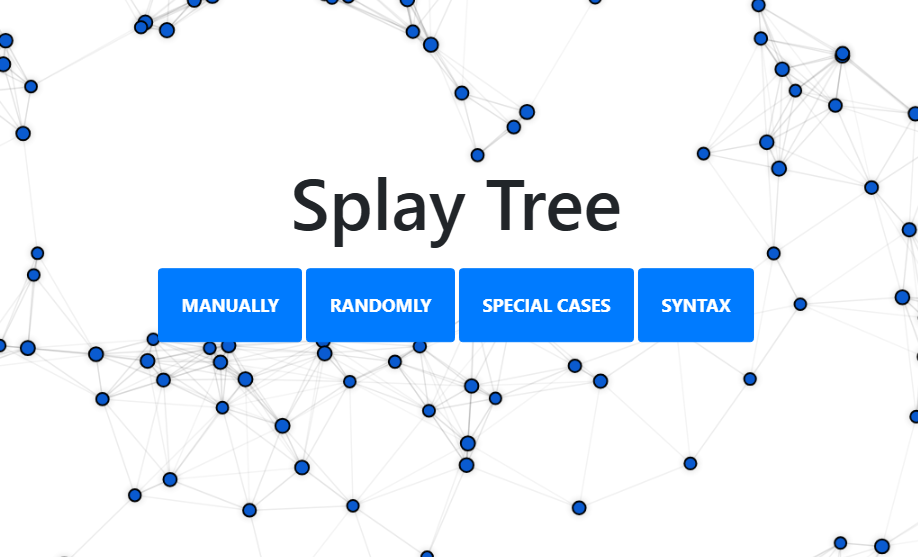
\includegraphics[width=0.9\textwidth]{Figures/input_modes_menu.png}
    \caption{Hlavní nabídka režimů zadávání vstupů u zvoleného algoritmu}
    \label{fig:input_modes_menu}
\end{figure}

Na obrázku \ref{fig:input_modes_menu} je znázorněna hlavní nabídka režimů zadávání vstupů, která je uživateli k dispozici po zvolení konkrétního algoritmu. Obrázek \ref{fig:input_modes_examples} pak ukazuje konkrétní podobu jednotlivých režimů zadávání, konkrétně ruční zadávání vstupů, náhodné generování, výběr nejlepšího nebo nejhoršího případu a zadávání vstupů pomocí syntaxe příkazů.

\begin{figure}[!h]
    \centering
    \subfloat[Ruční zadávání vstupů]{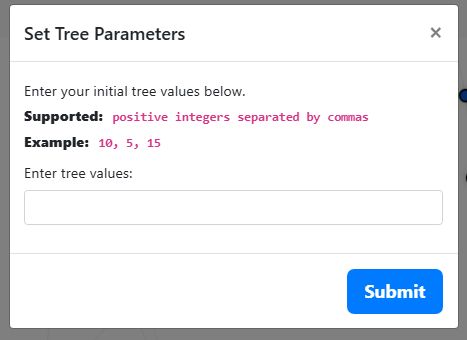
\includegraphics[width=0.45\textwidth]{Figures/input_manual.png}}
    \hfill
    \subfloat[Náhodné generování vstupů]{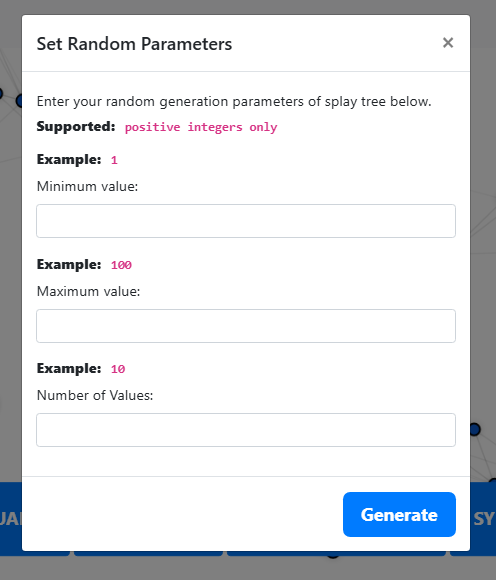
\includegraphics[width=0.45\textwidth]{Figures/input_random.png}} \\[0.5em]
    \subfloat[Volba nejlepšího/nejhoršího případu]{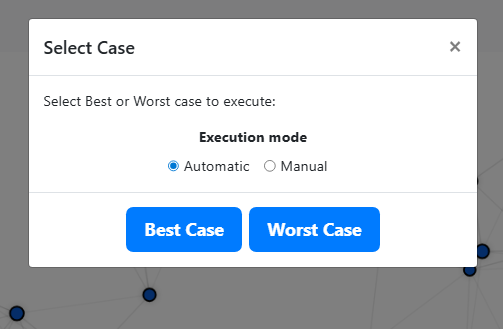
\includegraphics[width=0.45\textwidth]{Figures/input_bestworst.png}}
    \hfill
    \subfloat[Zadávání vstupů pomocí syntaxe příkazů]{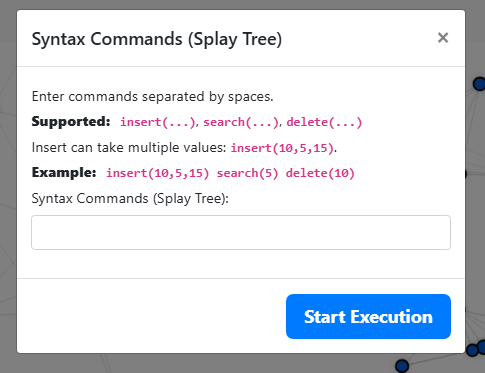
\includegraphics[width=0.45\textwidth]{Figures/input_syntax.png}}
    \caption{Příklady jednotlivých režimů zadávání vstupů}
    \label{fig:input_modes_examples}
\end{figure}

\newpage

\subsection{Zobrazení průběhu algoritmu po jednotlivých krocích}
Další důležitou součástí návrhu funkcionality komponenty bylo zobrazení průběhu algoritmu po jednotlivých krocích. Pro výuku amortizované složitosti totiž nestačí uživateli ukázat pouze konečný výsledek, ale je nutné umožnit mu sledovat, co se děje v průběhu celého výpočtu. Komponenta proto byla navržena tak, aby uživatel mohl vidět postupný vývoj algoritmu a změny stavu datové struktury v jednotlivých krocích simulace.

Takové zobrazení je důležité především proto, že studentovi umožňuje lépe pochopit návaznost jednotlivých operací a jejich vliv na další chování algoritmu. Díky krokovému průběhu lze sledovat nejen samotný výsledek operace, ale i způsob, jakým k němu algoritmus dospívá. Návrh této funkcionality proto představuje jednu z klíčových částí celé komponenty.

Na obrázku \ref{fig:syntax_step_mode} je znázorněn průběh algoritmu v režimu syntaxe, kde uživatel postupuje jednotlivými kroky simulace a může sledovat aktuální stav datové struktury i informace o právě prováděné operaci. Obrázek \ref{fig:bestworst_auto_mode} pak ukazuje automatický průběh v režimu nejlepšího/nejhoršího případu, kde se předem připravený scénář vykonává postupně bez nutnosti ručního zadávání každého kroku.

\begin{figure}[H]
    \centering
    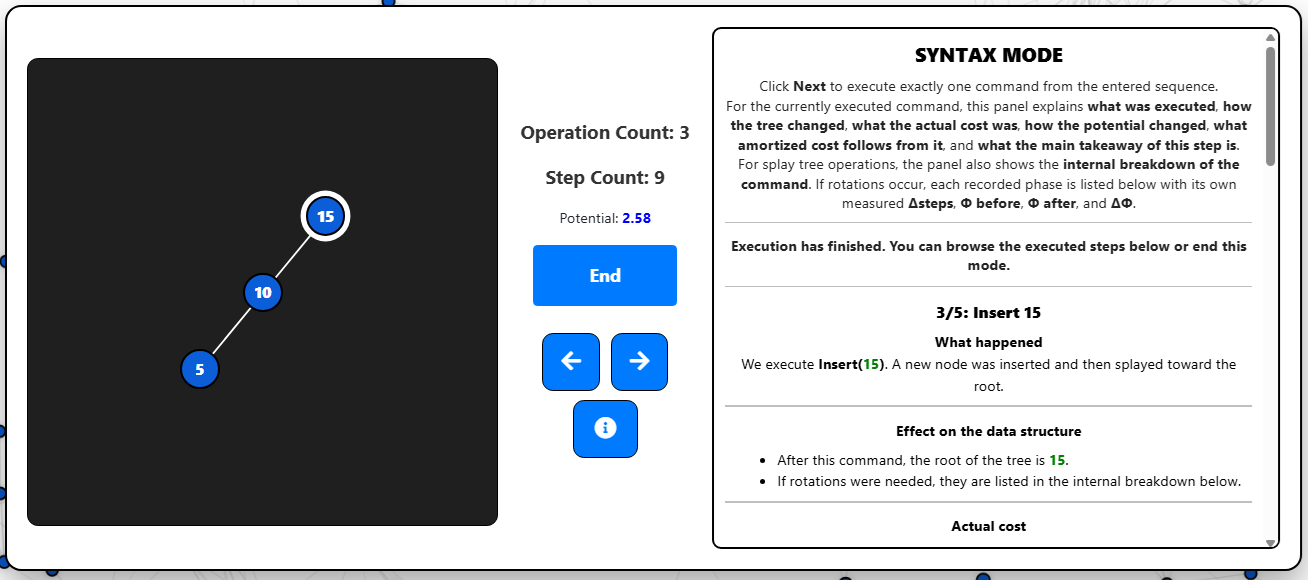
\includegraphics[width=0.95\textwidth]{Figures/syntax_step_mode.png}
    \caption{Zobrazení průběhu algoritmu po jednotlivých krocích v režimu syntaxe}
    \label{fig:syntax_step_mode}
\end{figure}

\begin{figure}[H]
    \centering
    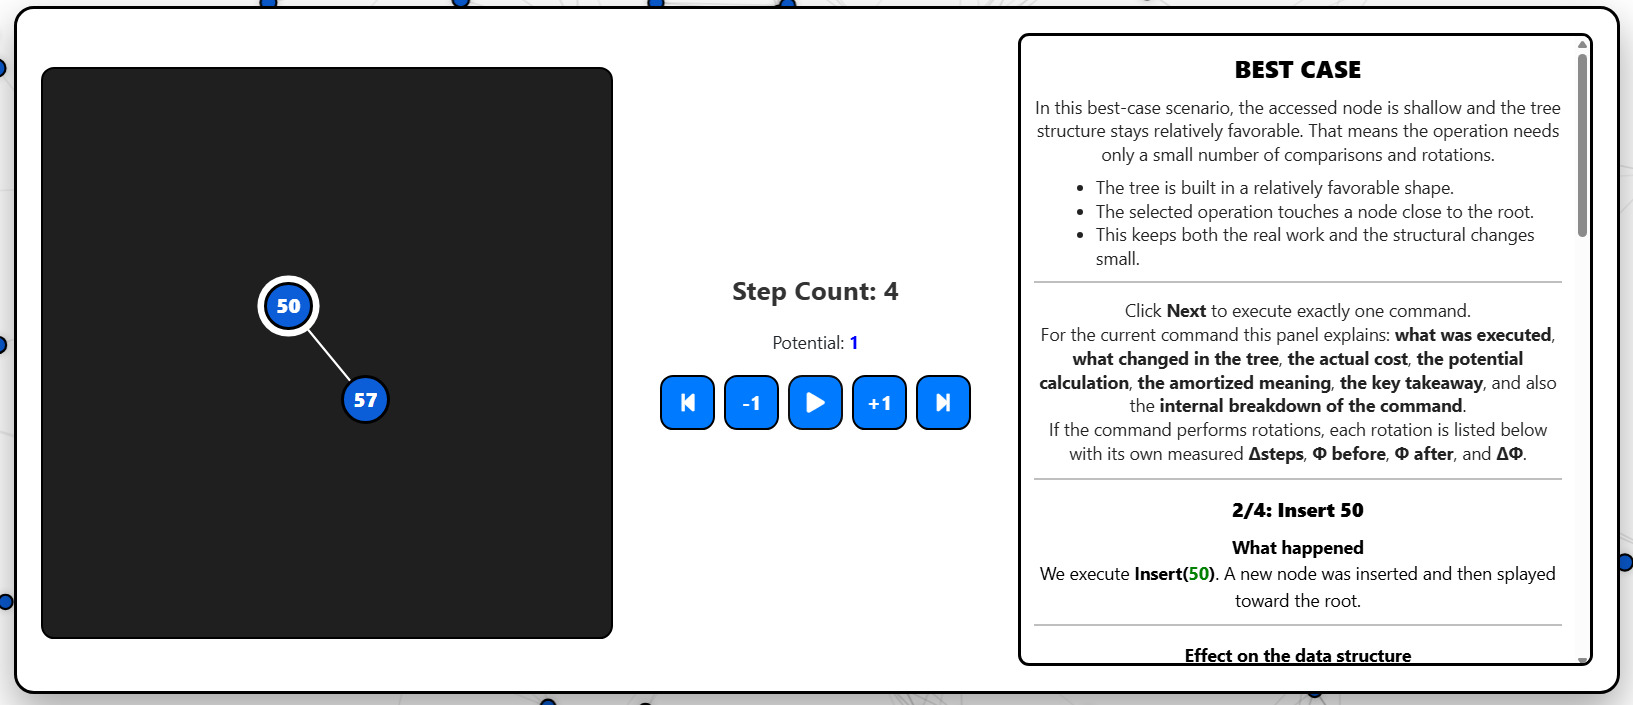
\includegraphics[width=0.95\textwidth]{Figures/bestworst_auto_mode.png}
    \caption{Automatický průběh simulace v režimu nejlepšího/nejhoršího případu}
    \label{fig:bestworst_auto_mode}
\end{figure}

\newpage

\subsection{Zobrazení počtu kroků a potenciálu}
Pro správné pochopení amortizované analýzy bylo při návrhu důležité zohlednit také zobrazení hodnot, které s tímto typem hodnocení přímo souvisejí. Komponenta proto měla zobrazovat počet provedených kroků a zároveň i hodnotu potenciálu, případně jinou odpovídající veličinu podle použité metody analýzy. Tyto hodnoty nemají sloužit pouze jako doplněk vizualizace, ale jako důležitá součást výkladu toho, proč se chování algoritmu hodnotí určitým způsobem.

Zobrazení počtu kroků a potenciálu umožňuje uživateli sledovat nejen to, co algoritmus právě vykonává, ale také to, jak se mění hodnoty důležité pro celkovou interpretaci jeho amortizované složitosti. Student tak může lépe pochopit vztah mezi jednotlivými operacemi, jejich skutečnými náklady a dlouhodobým chováním algoritmu v rámci celé posloupnosti operací.

Na obrázku \ref{fig:step_count_potential} je ukázáno zobrazení počtu provedených kroků a aktuální hodnoty potenciálu v průběhu simulace. Tyto informace jsou součástí hlavního rozhraní komponenty a tvoří důležitou oporu při sledování vývoje algoritmu i při interpretaci jeho amortizované složitosti.

\begin{figure}[H]
    \centering
    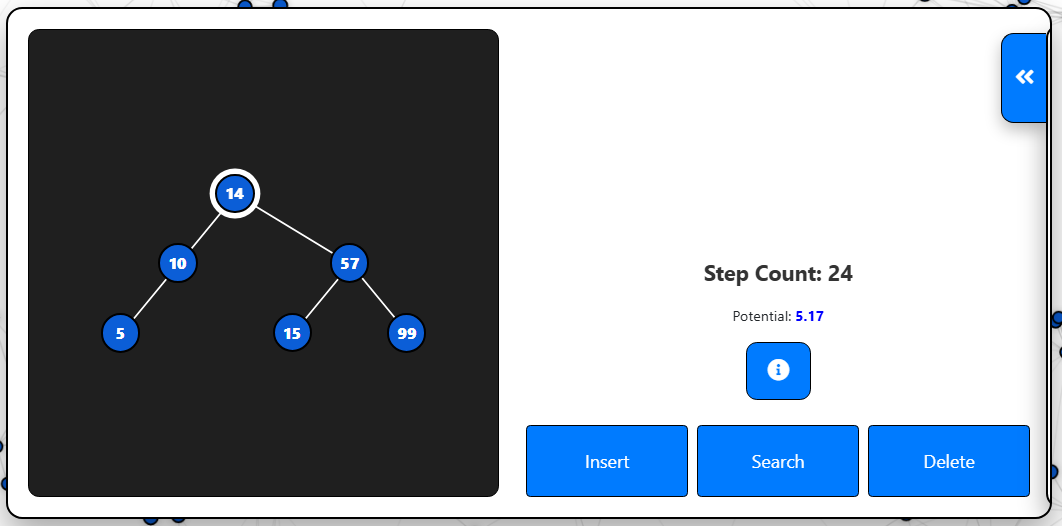
\includegraphics[width=0.95\textwidth]{Figures/step_count_potential.png}
    \caption{Zobrazení počtu kroků a aktuální hodnoty potenciálu v průběhu simulace}
    \label{fig:step_count_potential}
\end{figure}

\newpage

\subsection{Zobrazení doplňujících informací o aktuálním stavu algoritmu}
Součástí návrhu funkcionality komponenty bylo také zobrazení doplňujících informací o aktuálním stavu algoritmu. Samotná vizualizace datové struktury nebo zobrazení provedené operace totiž nemusí být vždy dostačující k tomu, aby uživatel přesně porozuměl tomu, co se v daném okamžiku děje. Z tohoto důvodu bylo vhodné doplnit průběh simulace o textové a přehledně uspořádané informace, které uživateli usnadní orientaci.

Tyto doplňující informace mají pomoci objasnit význam aktuálního kroku, stav datové struktury nebo souvislosti mezi právě prováděnou operací a chováním algoritmu jako celku. Uživatel tak nemá k dispozici pouze vizuální podobu aktuálního stavu, ale také slovní vysvětlení toho, co bylo provedeno, co se změnilo a jaký dopad má daný krok z hlediska amortizované analýzy. Návrh této části funkcionality tak podporuje srozumitelnost komponenty a přispívá k tomu, aby uživatel mohl lépe propojit vizuální průběh simulace s teoretickým výkladem algoritmu.

Na obrázku \ref{fig:history_info_panel} je znázorněn příklad detailních informací dostupných v historii vykonaných kroků. Obrázek \ref{fig:manual_info_panel} pak ukazuje doplňující informační panel přímo v průběhu práce s algoritmem, kde jsou zobrazeny informace vztahující se k aktuálně prováděné operaci.

\begin{figure}[H]
    \centering
    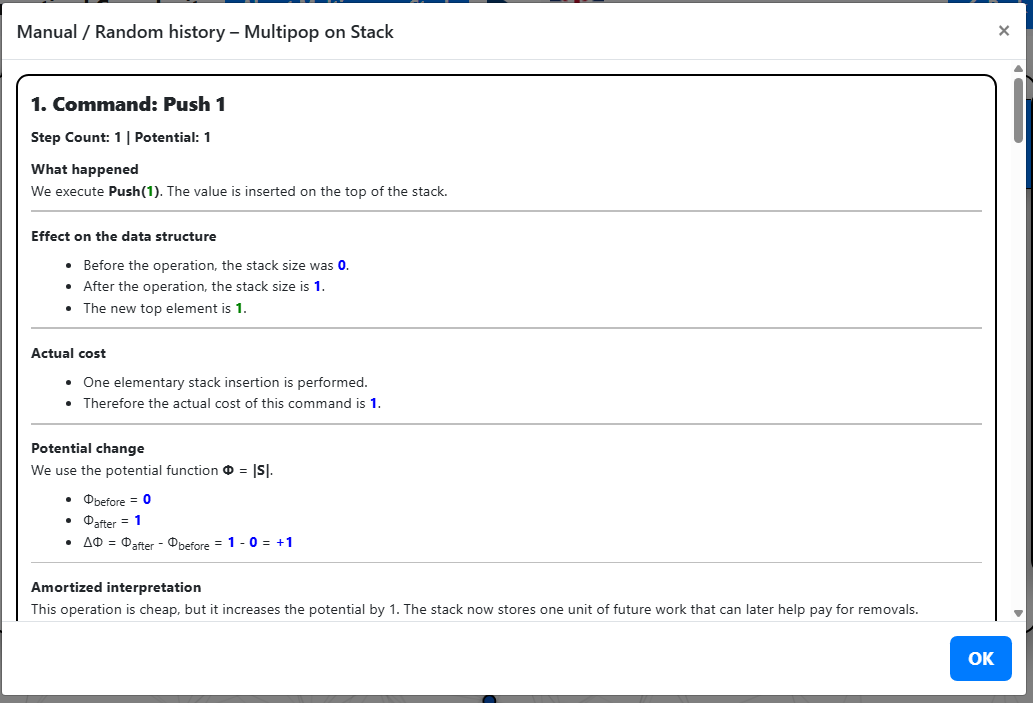
\includegraphics[width=0.92\textwidth]{Figures/history_info_panel.png}
    \caption{Detailní doplňující informace dostupné v historii provedených kroků}
    \label{fig:history_info_panel}
\end{figure}

\begin{figure}[H]
    \centering
    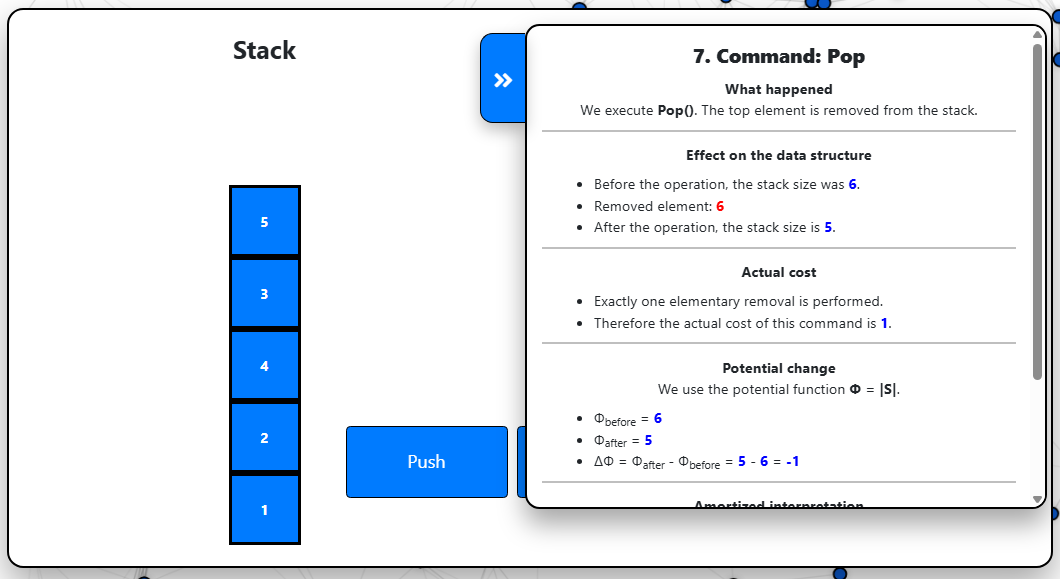
\includegraphics[width=0.92\textwidth]{Figures/manual_info_panel.png}
    \caption{Doplňující informační panel zobrazující aktuální stav operace při práci s algoritmem}
    \label{fig:manual_info_panel}
\end{figure}



\section{Návrh uživatelského rozhraní}
V této části je popsán návrh UI navrhované komponenty. Nejprve je pozornost věnována návrhu hlavní stránky a způsobu výběru jednotlivých algoritmů. Následně jsou shrnuty základní ovládací prvky simulace a způsob vizualizace použitých datových struktur. V závěru této části je popsán návrh informačních panelů a doprovodných vysvětlení, která mají podpořit výukový charakter komponenty.

\subsection{Návrh hlavní stránky a výběru algoritmu}
Při návrhu uživatelského rozhraní bylo důležité vytvořit hlavní stránku, která bude pro uživatele přehledná a umožní mu rychlou orientaci v celé komponentě. Hlavní stránka proto byla navržena jako výchozí rozcestník, z něhož si uživatel vybírá konkrétní algoritmus, se kterým chce dále pracovat. Současně bylo cílem, aby již na této úrovni bylo zřejmé, že komponenta slouží jako součást výukového prostředí zaměřeného na amortizovanou složitost.

Velký důraz byl kladen na jednoduchost výběru jednotlivých algoritmů. Uživatel má mít možnost z hlavní stránky přímo přejít k vybranému algoritmu, aniž by musel procházet složitější strukturu nabídek. Návrh proto počítal s výrazným zobrazením všech tří algoritmů zařazených do praktické části práce. Tím je zajištěno, že uživatel ihned vidí, jaké algoritmy jsou v komponentě dostupné, a může si zvolit ten, který chce právě vyzkoušet.

Součástí návrhu hlavní stránky byly také další prvky podporující orientaci a dostupnost informací. Patří mezi ně zejména možnost přepínání jazykových preferencí a přístup k doplňujícím informacím o samotné bakalářské práci. Hlavní stránka tak neslouží pouze jako technický vstup do aplikace, ale zároveň plní orientační a informační funkci.

Na obrázku \ref{fig:main_page_algorithm_selection} je znázorněna hlavní stránka komponenty, na níž jsou zobrazeny dostupné algoritmy, přepínač jazykových preferencí a tlačítko pro zobrazení informací o bakalářské práci.

\begin{figure}[H]
    \centering
    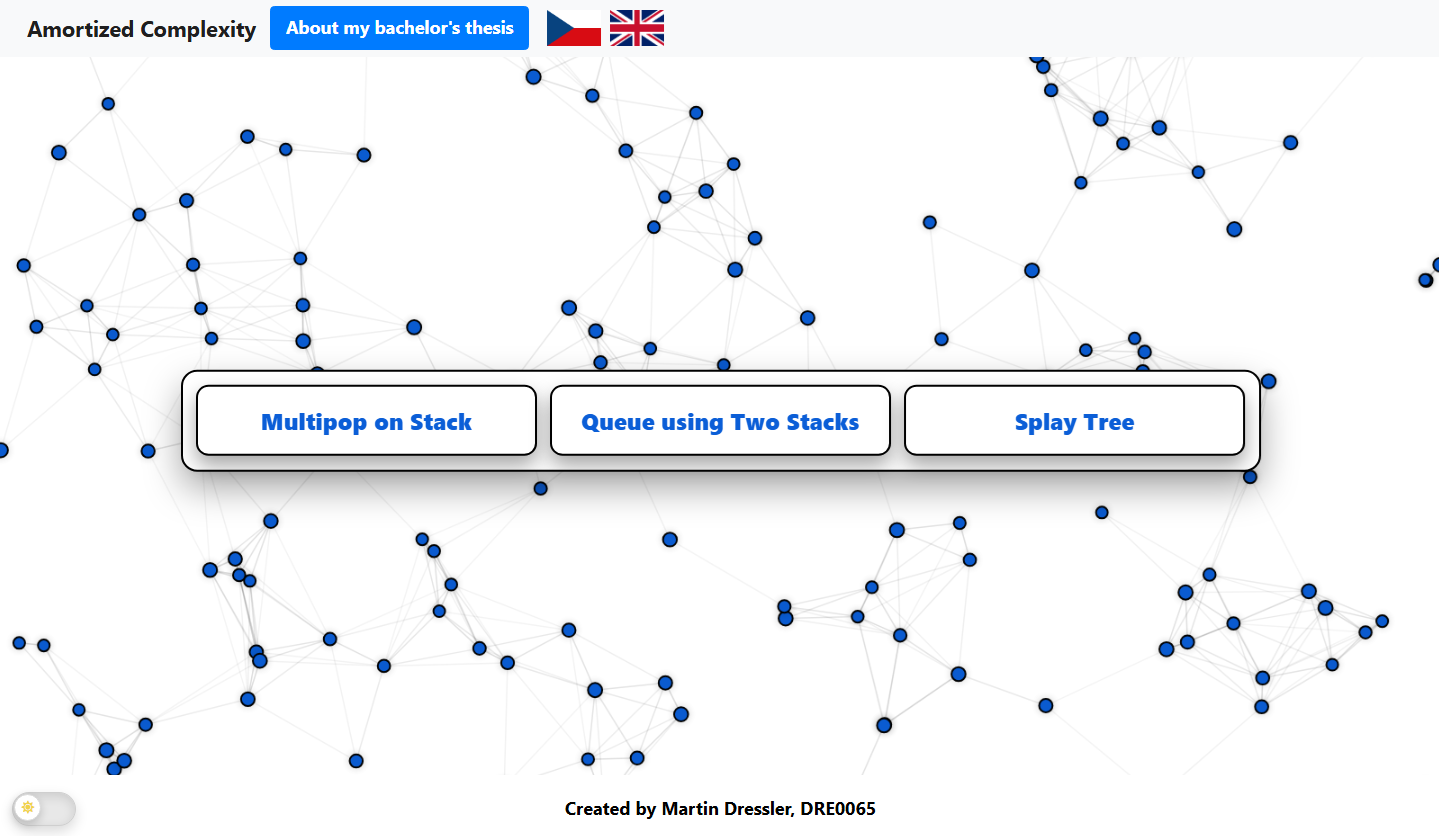
\includegraphics[width=0.95\textwidth]{Figures/main_page_algorithm_selection.png}
    \caption{Hlavní stránka komponenty s výběrem algoritmů, přepínačem jazykových mutací a tlačítkem pro informace o bakalářské práci}
    \label{fig:main_page_algorithm_selection}
\end{figure}

\subsection{Návrh ovládacích prvků simulace}
Součástí návrhu uživatelského rozhraní bylo také vytvoření vhodných ovládacích prvků simulace. Tyto prvky musely uživateli umožnit pohodlně řídit průběh algoritmu a současně podporovat srozumitelné sledování jednotlivých kroků. Návrh proto počítal s tím, že uživatel nebude pouze pasivně sledovat vykonávání algoritmu, ale bude moci průběh simulace aktivně ovlivňovat.

Důležitou součástí ovládání bylo zejména krokování mezi jednotlivými stavy simulace. Uživatel má mít možnost přecházet na předchozí nebo následující krok, ukončit aktuální režim a podle potřeby si zobrazit také doplňující historii informací. Ovládací prvky proto byly navrženy tak, aby byly snadno dostupné a přehledně oddělené od samotné vizualizace datové struktury. Tím je zajištěno, že uživatel může současně sledovat stav algoritmu i pohodlně pracovat s jeho ovládáním.

Na obrázku \ref{fig:simulation_controls} je znázorněn příklad návrhu ovládacích prvků simulace v režimu syntaxe. Součástí rozhraní jsou tlačítka pro pohyb mezi jednotlivými kroky, tlačítko pro ukončení režimu a tlačítko pro zobrazení historie informací.

\begin{figure}[H]
    \centering
    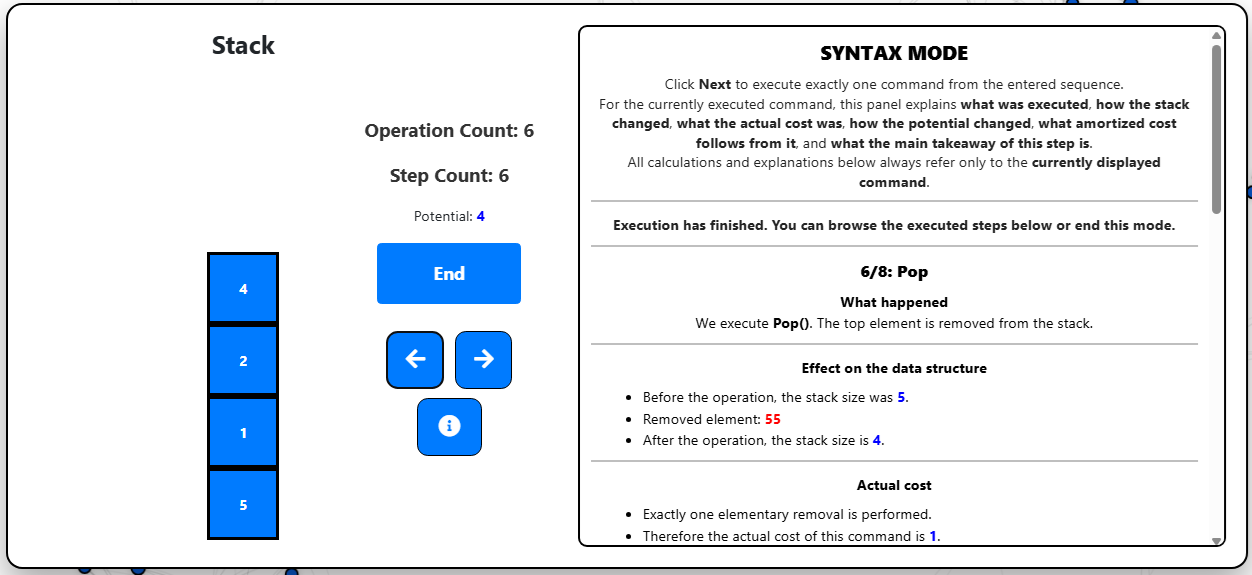
\includegraphics[width=0.95\textwidth]{Figures/simulation_controls.png}
    \caption{Příklad ovládacích prvků simulace v režimu syntaxe}
    \label{fig:simulation_controls}
\end{figure}

\subsection{Návrh vizualizace datových struktur}
Důležitou součástí návrhu uživatelského rozhraní bylo také zobrazení datových struktur používaných jednotlivými algoritmy. Cílem nebylo pouze zobrazit stav výpočtu formou číselných hodnot, ale navrhnout takovou vizualizaci, která uživateli umožní co nejlépe pochopit změny struktury v průběhu simulace. Z tohoto důvodu byla podoba vizualizace přizpůsobena konkrétnímu typu datové struktury, s níž daný algoritmus pracuje.

U algoritmu Multipop na zásobníku byla zvolena jednoduchá svislá reprezentace zásobníku, která přehledně ukazuje pořadí prvků i změny na vrcholu zásobníku. U fronty využívající dva zásobníky bylo naopak důležité oddělit oba zásobníky tak, aby bylo zřejmé, do které části se prvky vkládají a ze které se odebírají. U Splay stromu pak bylo nezbytné navrhnout stromovou vizualizaci, která umožní sledovat nejen obsah uzlů, ale i jejich vzájemné propojení a změny struktury při jednotlivých operacích.

Takto navržená vizualizace datových struktur podporuje názornost celé komponenty a umožňuje uživateli lépe porozumět tomu, jak se algoritmus chová při různých operacích. Uživatel tak nesleduje pouze výsledky výpočtu, ale i konkrétní změny uspořádání dat, které jsou pro pochopení amortizované složitosti důležité.

Na obrázku \ref{fig:data_structure_visualizations} jsou znázorněny příklady vizualizace datových struktur použitých v jednotlivých algoritmech, konkrétně zásobníku, fronty realizované pomocí dvou zásobníků a Splay stromu.

\begin{figure}[H]
    \centering
    \subfloat[Zásobník]{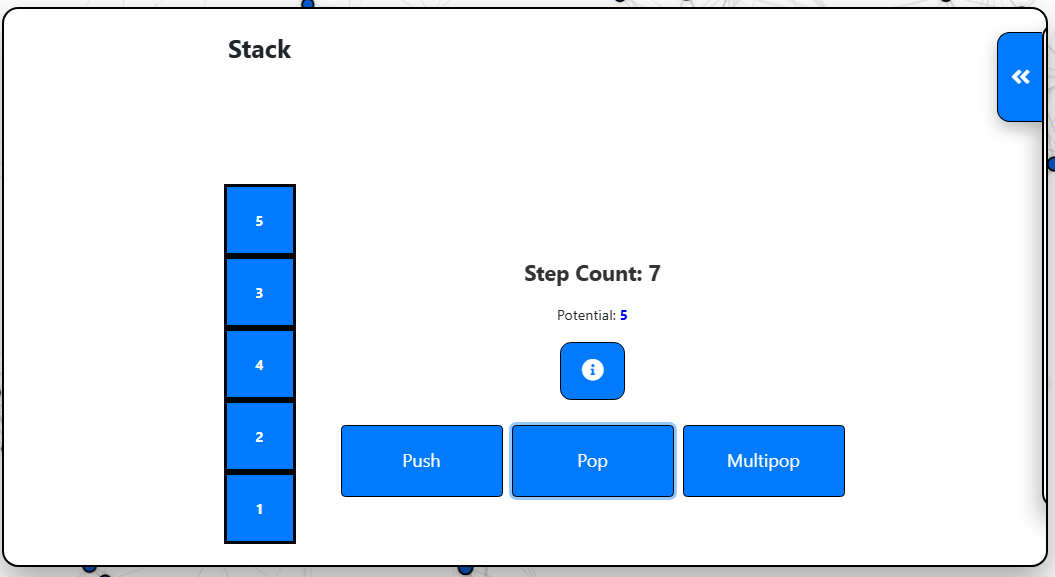
\includegraphics[width=0.6\textwidth]{Figures/stack_visualization.png}}
    \hfill
    \subfloat[Fronta využívající dva zásobníky]{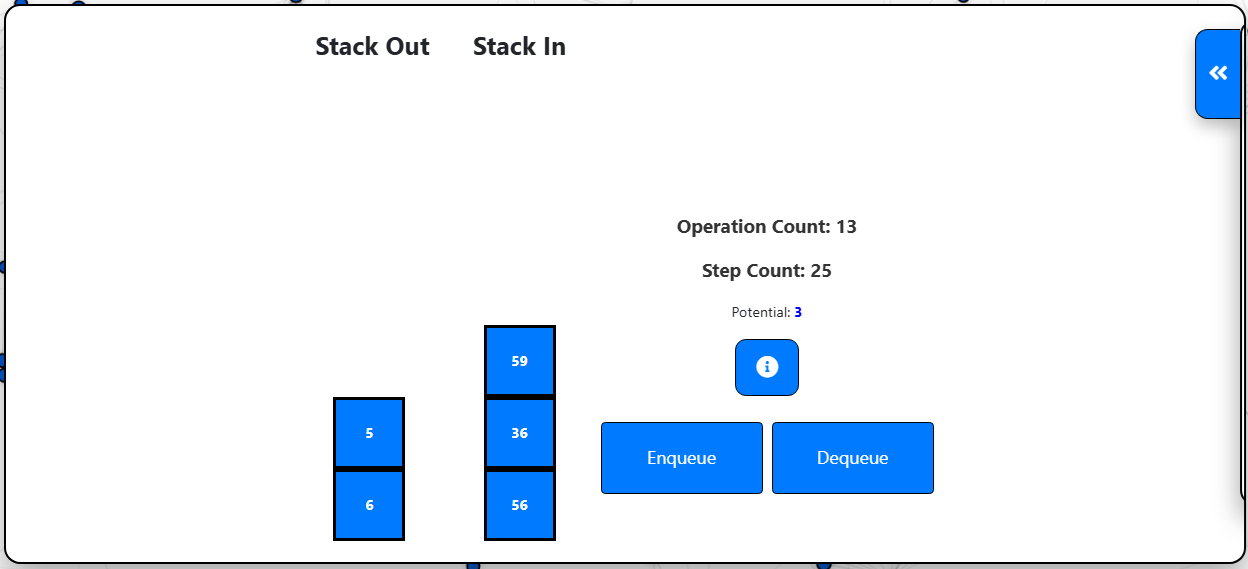
\includegraphics[width=0.6\textwidth]{Figures/queue_visualization.png}}
    \hfill
    \subfloat[Splay strom]{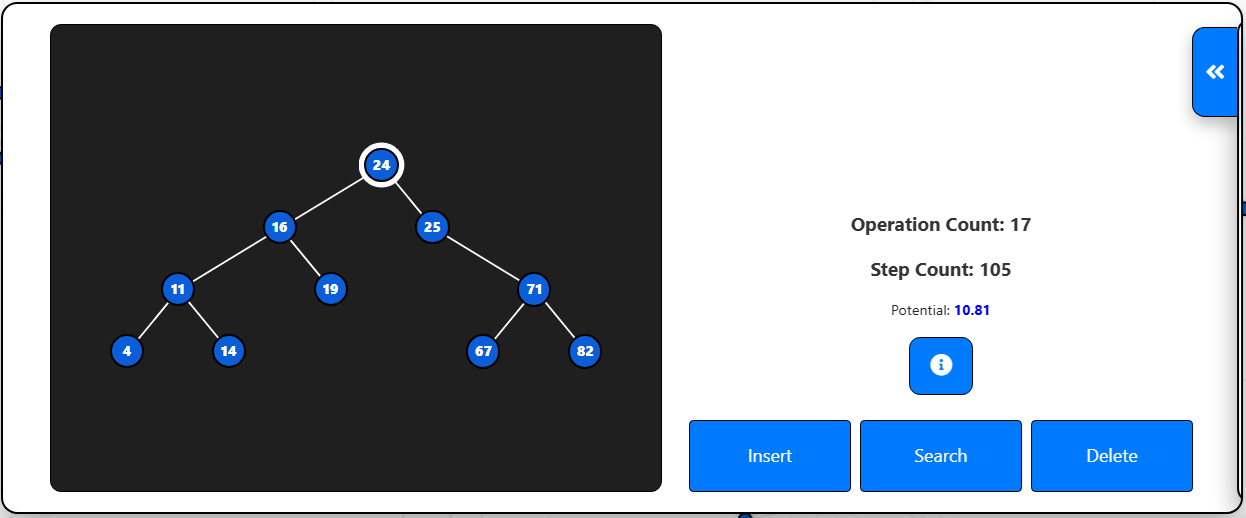
\includegraphics[width=0.6\textwidth]{Figures/splay_visualization.png}}
    \caption{Příklady vizualizace datových struktur použitých v navrhované komponentě}
    \label{fig:data_structure_visualizations}
\end{figure}

\subsection{Návrh informačních panelů a doprovodných vysvětlení o algoritmech}
Součástí návrhu uživatelského rozhraní byly také informační panely a doprovodná vysvětlení vztahující se k jednotlivým algoritmům. Cílem těchto částí rozhraní nebylo pouze doplnit simulaci o další text, ale nabídnout uživateli přehledné vysvětlení základních vlastností algoritmu, použitých operací a jeho vztahu k amortizované analýze. Díky tomu může uživatel získat potřebný teoretický kontext ještě před samotnou prací se simulací nebo v jejím průběhu.

Návrh těchto informačních panelů vycházel z potřeby propojit praktickou ukázku s doprovodným výkladem. Uživatel tak nemá k dispozici pouze vizualizaci datové struktury a ovládací prvky simulace, ale také souvislý popis algoritmu, jeho hlavní myšlenky a vysvětlení, proč je daný algoritmus vhodný pro amortizovanou analýzu. Takové řešení podporuje lepší orientaci v problematice a současně posiluje výukový charakter celé komponenty.

Na obrázku \ref{fig:algorithm_info_panel} je znázorněn příklad informačního panelu věnovaného jednomu z vybraných algoritmů. Panel obsahuje základní popis algoritmu, přehled jeho operací, hlavní princip fungování i stručné vysvětlení jeho složitosti z hlediska amortizované analýzy.

\begin{figure}[H]
    \centering
    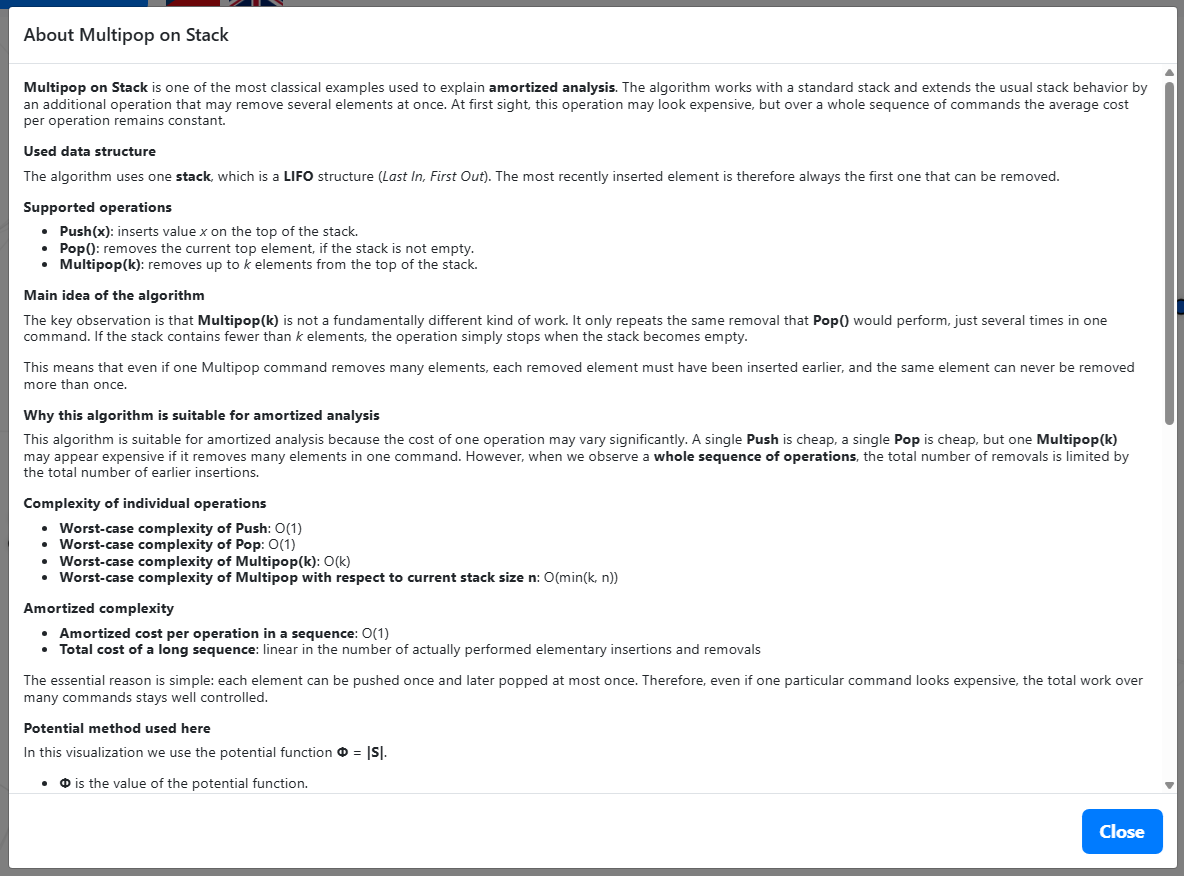
\includegraphics[width=0.95\textwidth]{Figures/algorithm_info_panel.png}
    \caption{Příklad informačního panelu s doprovodným vysvětlením vybraného algoritmu}
    \label{fig:algorithm_info_panel}
\end{figure}



\section{Návrh struktury komponenty}
Tato část se zaměřuje na návrh celkové struktury komponenty a na rozdělení jejích jednotlivých částí. Nejprve je popsáno oddělení společných prvků od částí specifických pro jednotlivé algoritmy. Následně je objasněna návaznost jednotlivých částí komponenty při práci uživatele. V závěru je pozornost věnována také možnostem budoucího rozšíření navrženého řešení.

\subsection{Rozdělení komponenty na společnou a algoritmicky specifickou část}
Celá struktura komponenty je rozdělena na prvky, které jsou společné pro všechny algoritmy, a na prvky, které jsou vytvořeny přímo pro konkrétní algoritmus. Mezi prvky patřící do společné části tvoří zejména hlavní stránka, výběr algoritmů, rozložení UI, obecné ovládací prvky a některé informační panely. Naopak část specifická pro daný algoritmus zahrnuje například samotnou logiku jednotlivých algoritmů, jejich konkrétní operace, způsob vizualizace příslušné datové struktury a doprovodné informace vztahující se k danému algoritmu. Díky tomuto rozdělení je možné zachovat jednotný vzhled a princip ovládání celé komponenty, ale zároveň ponechat dostatečný prostor pro přizpůsobení jednotlivým algoritmům.

\subsection{Návaznost jednotlivých částí komponenty}
Při návrhu byl brán zřetel také na návaznost jednotlivých částí z pohledu uživatele. Práce s komponentou začíná na hlavní stránce, kde si uživatel zvolí konkrétní algoritmus. Poté si vybere typ vstupu a sleduje průběh algoritmu, hodnoty důležité pro amortizovanou analýzu a doplňující vysvětlení. Jednotlivé části komponenty byly vytvořeny tak, aby na sebe logicky navazovaly a vytvářely ucelené prostředí pro práci uživatele.

\subsection{Možnosti budoucího rozšíření}
Při návrhu struktury bylo vhodné zohlednit také možnost budoucího rozšíření. Pokud by bylo potřeba aplikaci v budoucnu dále rozšířit, neměl by být problém přidat další algoritmy vhodné pro amortizovanou analýzu, aniž by bylo nutné zásadně měnit základní princip fungování celé komponenty. Stejným způsobem by bylo možné rozšiřovat informační panely, přidávat nové režimy práce se vstupy a další prvky.
\chapter{Implementace komponenty}
Navržená komponenta výukového serveru pro oblast TI byla realizována jako dynamická webová aplikace, která klade důraz na přehlednost, modularitu a interaktivní práci uživatele. Implementace vychází z rozdělení aplikace na samostatné logické celky, které zajišťují jak aplikační logiku, práci s~UI, tak i chování jednotlivých algoritmů. Důležitým aspektem tohoto řešení je propojení vizualizace s reálným průběhem výpočtu, kdy jsou jednotlivé kroky algoritmů přímo zobrazovány a aktualizovány prostřednictvím manipulace s DOM. Celá aplikace byla navržena tak, aby byla snadno rozšiřitelná, přehledná z pohledu implementace a zároveň vhodná pro praktické využití ve výuce.


\section{Použité technologie a vývojové prostředí}
Implementace komponenty byla realizována jako dynamická webová aplikace s využitím technologií HTML, CSS a JS. Jazyk HTML slouží pro definici struktury celé stránky, CSS pro její vizuální styl a responzivní zobrazení a JS pro zajištění aplikační logiky. Dynamická práce s obsahem stránky je realizována prostřednictvím manipulace s DOM, což umožňuje aktualizaci jednotlivých částí UI bez nutnosti opětovného načítání celé stránky. Pro vizuální animační efekty v pozadí stránky bylo využito také Canvas API \cite{canvas_api}.

V implementaci byly také využity vybrané knihovny, které usnadnily práci s UI. Pro stylování a~rozložení stránky byla použita knihovna Bootstrap \cite{bootstrap}, pro práci s ikonami knihovna Font Awesome \cite{font_awesome} a pro vybrané části klientské logiky knihovna jQuery \cite{jquery}. Aplikace nevyužívá žádné externí API, veškerá logika je realizována na straně klienta.

Celá praktická část byla vyvíjena v prostředí Visual Studio Code, které sloužilo pro implementaci aplikace. Teoretická část práce byla zpracována pomocí systému \LaTeX{} v prostředí Overleaf.


\section{Struktura a realizace aplikace}
Aplikace je rozdělena do více zdrojových souborů podle jejich účelu. Toto rozdělení zlepšuje přehlednost implementace, odděluje společné části od specializovaných modulů a usnadňuje další úpravy i~rozšiřování celé aplikace.

\subsection{Organizace zdrojových souborů}
Zdrojové soubory jsou rozděleny na hlavní stránku, sdílené prostředky, aplikační logiku, zpracování vstupních režimů a moduly jednotlivých algoritmů. Díky tomu lze snadno rozlišit, která část zajišťuje konkrétní chování aplikace.

\begin{itemize}
    \item \texttt{index.html} -- hlavní struktura stránky
    \item \texttt{styles.css} -- vzhled a responzivita
    \item \texttt{animation.js} -- animované pozadí stránky
    \item \texttt{translations.js} -- jazykové překlady aplikace
    \item \texttt{state\_app.js} -- globální stav aplikace
    \item \texttt{language\_app.js} -- přepínání jazyků
    \item \texttt{modals\_app.js} -- obsluha modálních oken
    \item \texttt{navigation\_app.js} -- navigace mezi částmi
    \item \texttt{theme\_app.js} -- vzhledové nastavení
    \item \texttt{init\_app.js} -- inicializace aplikace
    \item \texttt{helpers\_typesParams.js} -- pomocné funkce vstupů
    \item \texttt{manual\_typesParams.js} -- ruční zadávání vstupu
    \item \texttt{random\_typesParams.js} -- náhodné generování vstupu
    \item \texttt{specialCases\_typesParams.js} -- ukázkové speciální případy
    \item \texttt{syntax\_typesParams.js} -- vstup pomocí příkazů
    \item \texttt{state\_multipop.js} -- globální stav algoritmu Multipop na zásobníku
    \item \texttt{ui\_multipop.js} -- rozhraní algoritmu Multipop na zásobníku
    \item \texttt{manual\_multipop.js} -- ruční režim algoritmu Multipop na zásobníku
    \item \texttt{actions\_multipop.js} -- operace algoritmu Multipop na zásobníku
    \item \texttt{syntax\_multipop.js} -- syntaxe algoritmu Multipop na zásobníku
    \item \texttt{random\_multipop.js} -- náhodný režim algoritmu Multipop na zásobníku
    \item \texttt{specialCases\_multipop.js} -- speciální případy algoritmu Multipop na zásobníku
    \item \texttt{state\_queue2Stacks.js} -- globální stav algoritmu Fronta pomocí dvou zásobníků
    \item \texttt{ui\_queue2Stacks.js} -- rozhraní algoritmu Fronta pomocí dvou zásobníků
    \item \texttt{manual\_queue2Stacks.js} -- ruční režim algoritmu Fronta pomocí dvou zásobníků
    \item \texttt{actions\_queue2Stacks.js} -- operace algoritmu Fronta pomocí dvou zásobníků
    \item \texttt{syntax\_queue2Stacks.js} -- syntaxe algoritmu Fronta pomocí dvou zásobníků
    \item \texttt{random\_queue2Stacks.js} -- náhodný režim algoritmu Fronta pomocí dvou zásobníků
    \item \texttt{specialCases\_queue2Stacks.js} -- speciální případy algoritmu Fronta pomocí dvou zásobníků
    \item \texttt{state\_splayTree.js} -- globální stav algoritmu Splay strom
    \item \texttt{ui\_splayTree.js} -- rozhraní algoritmu Splay strom
    \item \texttt{manual\_splayTree.js} -- ruční režim algoritmu Splay strom
    \item \texttt{actions\_splayTree.js} -- operace algoritmu Splay strom
    \item \texttt{syntax\_splayTree.js} -- syntaxe algoritmu Splay strom
    \item \texttt{random\_splayTree.js} -- náhodný režim algoritmu Splay strom
    \item \texttt{specialCases\_splayTree.js} -- speciální případy algoritmu Splay strom
\end{itemize}

\subsection{Hlavní části aplikační logiky}
Velmi důležitou součástí implementace je hlavní aplikační logika, která zajišťuje propojení jednotlivých částí celé aplikace. Tato vrstva se stará zejména o správu globálního stavu, změny zobrazeného obsahu, aktualizaci rozhraní a návaznost mezi jednotlivými moduly. Právě díky této části aplikace spolu mohou správně spolupracovat sdílené prvky, jednotlivé algoritmy i různé režimy spuštění.

Jako ukázka hlavní aplikační logiky byla vybrána funkce \texttt{changeLanguage()}. Tato funkce se nachází v souboru \texttt{language\_app.js}. Její výběr je vhodný proto, že dobře ukazuje centrální řízení aplikace, protože při změně jazyka neaktualizuje pouze texty v rozhraní, ale také pracuje s uloženým nastavením, mění jazyk dokumentu, obnovuje aktuální zobrazení aplikace a zajišťuje správnou aktualizaci otevřených modálních oken i dalších aktivních prvků.

\begin{lstlisting}[language=Java, caption={Ukázka hlavní aplikační logiky ve funkci changeLanguage()}, label={lst:change_language}]
function changeLanguage(language){
  closeNavbarMenu();
  localStorage.setItem('language', language);
  document.documentElement.lang = language === 'cz' ? 'cs' : 'en';

  const Lall = trAll(language);

  langAppApplyCommonStaticTexts(Lall);
  langAppApplyAccessibilityTexts(Lall);
  langAppApplyAlgorithmSelectionTexts(Lall);
  langAppApplyPageTexts(language, Lall);
  langAppApplyParameterButtonTexts(Lall);
  langAppApplyManualModalTexts(Lall, language);
  langAppApplyRandomModalTexts(language, Lall);
  langAppApplySyntaxModalTexts(Lall);
  langAppApplySpecialCasesModalTexts(Lall);

  refreshCurrentViewAfterLanguageChange();
  langAppRefreshRandomOperationPreviews();

  if(typeof refreshOpenTransientModalsForLanguage === 'function')
    refreshOpenTransientModalsForLanguage();
  if(typeof refreshOpenSpecialCasesModalForLanguage === 'function')
    refreshOpenSpecialCasesModalForLanguage();
  if(typeof refreshOpenHistoryModalForLanguage === 'function')
    refreshOpenHistoryModalForLanguage();
  if(typeof updateThemeToggleUI === 'function')
    updateThemeToggleUI();
}
\end{lstlisting}
\addcontentsline{lof}{figure}{\protect\numberline{\thelstlisting}Ukázka hlavní aplikační logiky ve funkci changeLanguage()}

Na uvedené ukázce \ref{lst:change_language} je vidět, že hlavní aplikační logika není omezena jen na jednu dílčí činnost, ale propojuje více částí systému současně. Funkce nejprve uloží zvolený jazyk, následně upraví jazyk dokumentu a poté aktualizuje textové prvky celého rozhraní. Současně zajistí obnovení právě zobrazené části aplikace a případně i aktualizaci otevřených modálních oken nebo dalších aktivních prvků. Tento způsob řešení podporuje centralizaci důležité logiky na jednom místě a~zároveň usnadňuje správu i další rozšiřování aplikace.

\subsection{Implementace vybraných algoritmů}
V praktické části byly implementovány tři algoritmy: \textit{Multipop on Stack}, \textit{Queue using Two Stacks} a \textit{Splay Tree}. Každý z nich reprezentuje jiný typ chování vhodný pro amortizovanou analýzu. První algoritmus pracuje se zásobníkem založeným na principu LIFO, druhý simuluje frontu s principem FIFO pomocí dvou zásobníků a třetí algoritmus vychází z vlastností binárního vyhledávacího stromu BST, který se při operacích dynamicky přizpůsobuje. Z důvodu přehlednosti nejsou v této podkapitole uvedeny celé implementace algoritmů, ale pouze vybrané a zkrácené ukázky kódu, na kterých je dobře vidět hlavní princip jejich realizace.

Jako první ukázka byla vybrána část implementace algoritmu \textit{Multipop on Stack}, konkrétně operace \texttt{multipopFromStackManual(count)} ze souboru \texttt{manual\_multipop.js}. Tato ukázka byla zvolena proto, že přímo vystihuje hlavní princip algoritmu, tedy odebrání více prvků ze zásobníku najednou, přičemž skutečný počet odebraných prvků závisí na aktuálním stavu zásobníku.

\begin{lstlisting}[language=Java, caption={Zkrácená ukázka implementace operace multipop}, label={lst:multipop_impl}]
function multipopFromStackManual(count){
  if(mpBusy)
    return null;

  const beforeState = mpCreateStateSnapshot();
  const actualCount = Math.min(count, beforeState.size);

  if(actualCount === 0)
    return [];

  const removedValues = beforeState.snapshot.slice(-actualCount);
  const afterSnapshot = beforeState.snapshot.slice(0, beforeState.size - actualCount);

  mpApplyManualStateAndRefresh(
    afterSnapshot,
    beforeState.stepCount + actualCount,
    afterSnapshot.length
  );

  return removedValues;
}
\end{lstlisting}
\addcontentsline{lof}{figure}{\protect\numberline{\thelstlisting}Zkrácená ukázka implementace operace multipop}

Na ukázce \ref{lst:multipop_impl} je vidět, že implementace nejprve zjistí aktuální stav zásobníku a následně určí skutečný počet prvků, které lze odebrat. Ten je omezen minimem mezi požadovaným počtem a aktuální velikostí zásobníku. Právě tato vlastnost dobře vystihuje rozdíl mezi požadovanou a skutečně provedenou prací, což je pro tento algoritmus z hlediska amortizované analýzy podstatné.

Jako druhá ukázka byla vybrána část implementace algoritmu \textit{Queue using Two Stacks}. Konkrétně jde o funkci \texttt{qTransferAllFromInToOut(done)} ze souboru \texttt{manual\_queue2Stacks.js}. Tato ukázka byla zvolena proto, že zachycuje klíčový mechanismus celé struktury, tedy přesun prvků ze vstupního zásobníku do výstupního zásobníku.

\begin{lstlisting}[language=Java, caption={Zkrácená ukázka přesunu prvků při implementaci fronty pomocí dvou zásobníků}, label={lst:queue_transfer_impl}]
function qTransferAllFromInToOut(done){
  if(qIn.length === 0){
    qPotential = qIn.length;
    updateQueueCounters();
    
    if(done)
      done();
    return;
  }

  const value = qIn[qIn.length - 1];
  qAnimateRemoveTopItem('qInView', () => {
    qIn.pop();
    qStepCount += 1;

    qOut.push(value);
    qStepCount += 1;
    qPotential = qIn.length;
    
    renderQueueStacks();
    qAnimateAddTopItem('qOutView');
    updateQueueCounters();

    qRunTimer = setTimeout(() => {
      qTransferAllFromInToOut(done);
    }, qSkipAnimations ? 0 : 250);
  });
}
\end{lstlisting}
\addcontentsline{lof}{figure}{\protect\numberline{\thelstlisting}Zkrácená ukázka přesunu prvků při implementaci fronty pomocí dvou zásobníků}

Ukázka \ref{lst:queue_transfer_impl} vystihuje princip, na kterém je založena realizace fronty pomocí dvou zásobníků. Pokud je výstupní zásobník prázdný, prvky se postupně přesouvají ze vstupního zásobníku, čímž dojde k obrácení jejich pořadí. Právě tímto způsobem je možné zajistit chování odpovídající principu FIFO, přestože vnitřně aplikace pracuje se dvěma zásobníky.

Jako třetí ukázka byla vybrána část implementace algoritmu \textit{Splay Tree}, konkrétně funkce \texttt{sRotateLeft(node)} ze souboru \texttt{manual\_splayTree.js}. Tato ukázka byla zvolena proto, že rotace představují základní mechanismus, pomocí kterého se splay strom při operacích strukturálně upravuje.

\begin{lstlisting}[language=Java, caption={Zkrácená ukázka levé rotace ve splay stromu}, label={lst:splay_rotate_left}]
function sRotateLeft(node){
  const rightChild = node.right;
  if(!rightChild)
    return;

  sStepCount += 1;

  node.right = rightChild.left;
  if(rightChild.left)
    rightChild.left.parent = node;

  rightChild.parent = node.parent;

  if(!node.parent)
    sRoot = rightChild;
  else if(node === node.parent.left)
    node.parent.left = rightChild;
  else
    node.parent.right = rightChild;

  rightChild.left = node;
  node.parent = rightChild;
}
\end{lstlisting}
\addcontentsline{lof}{figure}{\protect\numberline{\thelstlisting}Zkrácená ukázka levé rotace ve splay stromu}

Na ukázce \ref{lst:splay_rotate_left} je vidět, jak se při levé rotaci mění vazby mezi vrcholy stromu. Přestože jde jen o zkrácenou část implementace, dobře ukazuje, že splay strom není založen pouze na běžném vyhledávání ve struktuře BST, ale také na dynamické změně jejího tvaru pomocí rotací. Právě tyto strukturální úpravy jsou pro chování splay stromu a jeho amortizovanou analýzu zásadní.

\subsection{Zpracování vstupů a režimů spuštění}
Důležitou součástí implementace je také zpracování vstupů a jednotlivých režimů spuštění aplikace. Uživatel může pracovat s několika způsoby zadání, konkrétně ručním vstupem, náhodně generovaným vstupem, vstupem pomocí syntaxe a připravenými speciálními případy. Pro přehlednost a znovupoužitelnost byla tato část řešena pomocí společné vrstvy \texttt{typesParams}, která sjednocuje obsluhu jednotlivých typů vstupů pro všechny implementované algoritmy.

Jako ukázka zpracování vstupů a režimů spuštění byla vybrána zkrácená část konfigurace. Konkrétně jde o \texttt{ALG\_REGISTRY}. Ukázka přehledně zachycuje, jak jsou pro jednotlivé algoritmy definovány dostupné režimy spuštění. Současně je na ní vidět, jak je nad těmito režimy vystavěna společná obslužná vrstva. Z ukázky je také patrné, že aplikace neřeší každý algoritmus zcela samostatně, ale používá jednotný princip pro ruční vstup, náhodné generování, speciální případy i syntax režim.

\begin{lstlisting}[language=Java, basicstyle=\ttfamily\scriptsize, breaklines=true, columns=fullflexible, caption={Zkrácená ukázka konfigurace vstupních režimů}, label={lst:types_params_registry}]
const ALG_REGISTRY = Object.freeze({
  multipop: {
    contexts: {manual: 'multipopManual', random: 'multipopRandom', specialCases: 'multipopSpecialCases', syntax: 'multipopSyntax'},
    manual: {type: 'stackModal', start: typesParamsStartMultipopWithValues},
    random: {type: 'randomModal', start: typesParamsStartMultipopRandomMode},
    specialCases: {getScenarios: typesParamsGetMultipopSpecialScenarios, start: typesParamsRunMultipopSpecialScenario},
    syntax: {resetBeforeOpen: typesParamsResetMultipopSyntaxState, start: typesParamsStartMultipopSyntax}
  },
  queue2Stacks: {
    contexts: {manual: 'queueManual', random: 'queueRandom', specialCases: 'queueSpecialCases', syntax: 'queueSyntax'},
    manual: {type: 'stackModal', start: typesParamsStartQueueWithValues},
    random: {type: 'randomModal', start: typesParamsStartQueueRandomMode},
    specialCases: {getScenarios: typesParamsGetQueueSpecialScenarios, start: typesParamsRunQueueSpecialScenario},
    syntax: {resetBeforeOpen: typesParamsResetQueueSyntaxState, start: typesParamsStartQueueSyntax}
  },
  splayTree: {
    contexts: {manual: 'splayManual', random: 'splayRandom', specialCases: 'splaySpecialCases', syntax: 'splaySyntax'},
    manual: {type: 'actionInput', titleKey: 'splayInitTitle', labelKey: 'splayInitLabel', infoKey: 'splayInitInfo', invalidKey: 'splayInitInvalid', start: typesParamsStartSplayManualWithValues},
    random: {type: 'randomModal', start: typesParamsStartSplayRandomMode},
    specialCases: {getScenarios: typesParamsGetSplaySpecialScenarios, start: typesParamsRunSplaySpecialScenario},
    syntax: {start: typesParamsStartSplaySyntax}
  }
});
\end{lstlisting}
\addcontentsline{lof}{figure}{\protect\numberline{\thelstlisting}Zkrácená ukázka konfigurace vstupních režimů}

Na ukázce \ref{lst:types_params_registry} je vidět, že vrstva \texttt{typesParams} sjednocuje obsluhu všech hlavních režimů spuštění aplikace. Pro každý algoritmus jsou zde definovány kontexty jednotlivých režimů, tedy manuální vstup, náhodný vstup, speciální případy a syntax režim. Současně je zde určeno, jaký typ vstupního rozhraní se má použít a která funkce zajistí samotné spuštění zvoleného režimu. Toto řešení přispívá k větší modularitě aplikace, protože společná logika zpracování vstupů není duplikována v každém algoritmu zvlášť. Vrstva \texttt{typesParams} tak tvoří rozhraní mezi uživatelským zadáním a konkrétní implementací jednotlivých algoritmů.


\section{Uživatelské rozhraní a responzivita}
UI je důležitou částí celé aplikace, protože zprostředkovává práci s algoritmy, vstupy i jednotlivými režimy spuštění. Současně bylo nutné navrhnout jej tak, aby zůstalo přehledné při dynamických změnách obsahu a bylo použitelné i na různých typech zařízení.

\subsection{Struktura uživatelského rozhraní a práce s dynamickým obsahem}
Součástí implementace je návrh struktury UI a způsob, jakým je do stránky vkládán a měněn dynamický obsah. Aplikace není vytvořena jako sada více samostatných statických stránek, ale jako jedna hlavní dynamická stránka, ve které se podle zvoleného algoritmu a režimu spuštění mění zobrazovaný obsah přímo v rámci DOM.

Jako ukázka byla vybrána zkrácená část HTML struktury z těla dokumentu. Tato ukázka pochází ze souboru \texttt{index.html}. Přehledně zachycuje hlavní navigaci, výběr algoritmů, prostor pro dynamicky vkládaný obsah, modální okna i další prvky rozhraní.

\begin{lstlisting}[language=XML, basicstyle=\ttfamily\scriptsize, breaklines=true, columns=fullflexible]
<body>
  <canvas id="bgCanvas" aria-hidden="true"></canvas>
  
  <!-- Hlavni navigace -->
  <nav class="navbar ..." >
    ...
    <button id="aboutAppBtn" ...>...</button>
    <div id="backArrow">
      <button id="backBtn" ...>...</button>
    </div>
  </nav>
  
  <!-- Vyber algoritmu -->
  <div class="alg-panel" id="algorithmLinks">
    ...
    <button id="algorithm1" onclick="changeContent('multipop')">...</button>
    <button id="algorithm2" onclick="changeContent('queue2Stacks')">...</button>
    <button id="algorithm3" onclick="changeContent('splayTree')">...</button>
  </div>

  <!-- Dynamicky obsah -->
  <div id="dynamicContent" class="text-center mt-5"></div>
\end{lstlisting}
\newpage
\noindent\textit{Pokračování ukázky kódu.}
\begin{lstlisting}[language=XML, basicstyle=\ttfamily\scriptsize, breaklines=true, columns=fullflexible, caption={Zkrácená ukázka struktury uživatelského rozhraní v souboru index.html}, label={lst:index_body_ui}]
  <!-- Priklad modalniho okna -->
  <div class="modal fade" id="aboutModal" ...>
    <div class="modal-dialog ...">
      <div class="modal-content">
        <div class="modal-header">
          <h5 id="aboutModalLabel"></h5>
        </div>
        <div class="modal-body" id="aboutModalBody"></div>
        <div class="modal-footer">
          <button id="closeBtn" ...></button>
        </div>
      </div>
    </div>
  </div>

  <!-- Dalsi modalni okna -->
  ...
  <footer>
    ...
    <button id="themeToggle" class="theme-toggle"></button>
    <span id="footerText"></span>
  </footer>

  <!-- Nacteni JS souboru -->
  <script src="..."></script>
  ...
</body>
\end{lstlisting}
\phantomsection
\addcontentsline{lof}{figure}{\protect\numberline{\thelstlisting}Zkrácená ukázka struktury uživatelského rozhraní v souboru index.html}

Na ukázce \ref{lst:index_body_ui} je vidět, že uživatelské rozhraní je postaveno na jedné společné HTML kostře. Ta obsahuje hlavní navigaci, úvodní panel pro výběr algoritmů, centrální prvek \texttt{dynamicContent} určený pro dynamicky vkládaný obsah, sadu modálních oken a také patičku s dalšími ovládacími prvky. Právě element \texttt{dynamicContent} slouží jako hlavní prostor, do kterého aplikace podle aktuální situace vkládá nové části rozhraní. Současně je z ukázky patrné, že důležitou roli hrají i modální okna, která slouží pro zadávání vstupních parametrů, zobrazení doplňujících informací nebo práci s historií kroků. Významná je také návaznost na načítané JS soubory.
\newpage

\subsection{Responzivní zobrazení na různých zařízeních}
V průběhu návrhu celé aplikace byl brán ohled také na responzivní zobrazení na mobilních zařízeních, i když tato část nebyla přímo požadována v zadání. Cílem bylo, aby aplikace zůstala použitelná a přehledná nejen na běžném monitoru, ale i na menších obrazovkách.

Na obrázku \ref{fig:responsive_ui_compare} je zachyceno porovnání hlavní stránky na desktopovém a mobilním zařízení. Ze srovnání je patrné, že aplikace si zachovává stejné základní prvky rozhraní, ale jejich rozmístění a velikost se přizpůsobují dostupnému prostoru obrazovky.

\begin{figure}[H]
    \centering
    \subfloat[Hlavní stránka aplikace na desktopovém zařízení]{%
        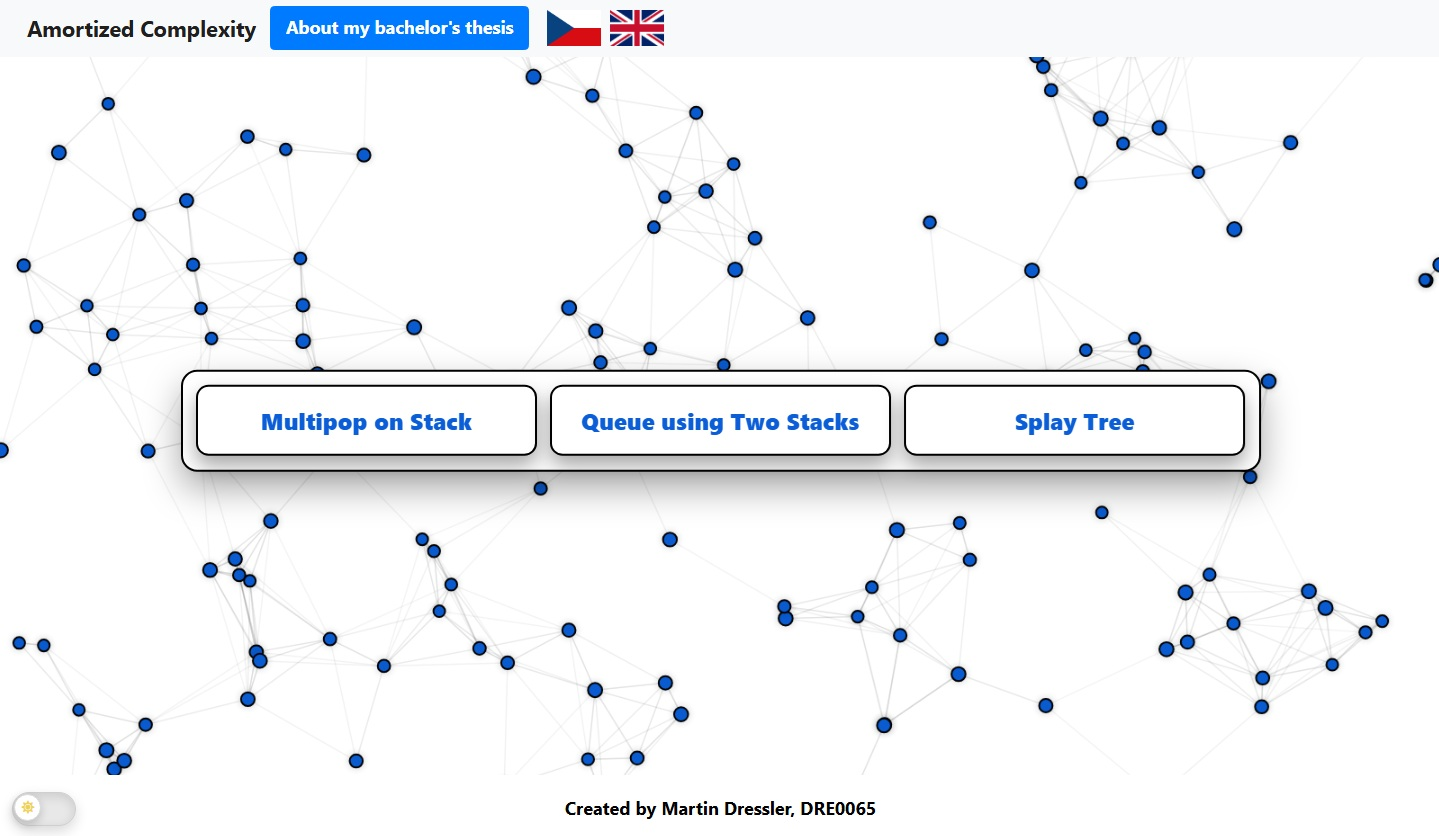
\includegraphics[width=0.7\textwidth]{Figures/main_page_algorithm_selection.jpg}}
    \hfill
    \subfloat[Hlavní stránka aplikace na mobilním zařízení]{%
        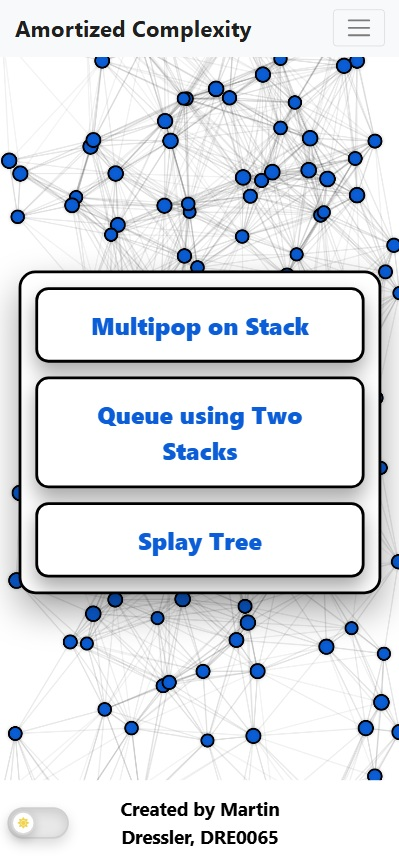
\includegraphics[width=0.3\textwidth]{Figures/mobile_main_page.jpg}}
    \caption{Porovnání zobrazení hlavní stránky na různých typech zařízení}
    \label{fig:responsive_ui_compare}
\end{figure}
\newpage

Responzivní chování bylo řešeno v souboru \texttt{styles.css} pomocí pravidel \texttt{@media}.

\begin{lstlisting}[basicstyle=\ttfamily\footnotesize, breaklines=true, columns=fullflexible, caption={Zkrácená ukázka responzivních pravidel pro mobilní zařízení}, label={lst:responsive_media_query}]
@media(max-width: 767.98px){
  ...
}
\end{lstlisting}
\addcontentsline{lof}{figure}{\protect\numberline{\thelstlisting}Zkrácená ukázka responzivních pravidel pro mobilní zařízení}

Na ukázce \ref{lst:responsive_media_query} je vidět, že pro menší obrazovky byla použita samostatná část stylů, která upravuje zobrazení aplikace pro mobilní zařízení. Díky tomu bylo možné zachovat přehlednost rozhraní i při výrazně menším dostupném prostoru.


\section{Nasazení a zpřístupnění aplikace}
Po dokončení implementace byla aplikace nasazena a zpřístupněna prostřednictvím školního serveru Homel, který se jevil jako nejvhodnější řešení pro hosting. Díky tomu je možné práci snadno veřejně zpřístupnit v rámci univerzitního prostředí a současně je zajištěn jednoduchý způsob, jak aplikaci prezentovat, testovat a dále využívat.

Pro spuštění aplikace není potřeba instalovat žádné další balíčky ani knihovny. Pro správnou funkci je nutné zachovat původní strukturu odevzdané praktické části, zejména adresáře \texttt{css}, \texttt{html}, \texttt{images} a \texttt{js}, protože aplikace využívá relativní cesty mezi soubory. Pro lokální spuštění stačí otevřít soubor \texttt{index.html} z adresáře \texttt{html} ve webovém prohlížeči. Knihovny Bootstrap, Font Awesome a~jQuery jsou připojeny prostřednictvím CDN, takže při spuštění je potřeba internetové připojení, aby se tyto prostředky mohly načíst. Není třeba upravovat žádné konfigurační soubory ani provádět sestavení aplikace, protože veškerá logika je realizována na straně klienta.

Výsledná aplikace je v době odevzdání bakalářské práce dostupná prostřednictvím protokolu HTTP na adrese URL \url{https://homel.vsb.cz/~dre0065/DRE0065_BP/html/}.
\chapter{Závěr}
Hlavním cílem této bakalářské práce bylo vytvořit komponentu výukového serveru pro oblast amortizované složitosti, která by budoucím studentům usnadnila pochopení tohoto tématu pomocí názorné a interaktivní vizualizace. V praktické části byla navržena a implementována webová aplikace umožňující práci s vybranými algoritmy vhodnými pro amortizovanou analýzu. Konkrétně byly zpracovány algoritmy Multipop on Stack, Queue using Two Stacks a Splay Tree, u nichž je možné sledovat jednotlivé kroky, změny stavů datových struktur i další hodnoty důležité pro pochopení jejich chování.

Součástí práce bylo také navržení struktury celé aplikace, zpracování různých typů vstupů, vytvoření uživatelského rozhraní a řešení responzivního zobrazení na různých typech zařízení. V~teoretické části byly popsány základní pojmy související s amortizovanou složitostí i hlavní části implementace navržené komponenty.

Výsledkem práce je funkční výukový nástroj, který může sloužit jako podpora při výuce i samostatném studiu a který může být v budoucnu rozšířen o další algoritmy. Současně tato práce shrnuje důležité informace o amortizované složitosti, vybraných algoritmech i samotné implementaci komponenty, které jsou popsány v tomto dokumentu ve formátu PDF.

\printbibliography[title={Literatura}, heading=bibintoc]

\appendix
\chapter{Obsah přiloženého ZIP souboru}

Součástí bakalářské práce je také elektronická příloha odevzdaná ve formě ZIP souboru.

\begin{table}[H]
\centering
\renewcommand{\arraystretch}{1.15}
\begin{tabular}{|L{0.30\textwidth}|L{0.62\textwidth}|}
\hline
\textbf{Název souboru / adresáře} & \textbf{Popis} \\
\hline
\texttt{DRE0065\_BP/} & Adresář obsahující praktickou část bakalářské práce, tedy zdrojové soubory webové aplikace určené k lokálnímu spuštění. \\
\hline
\texttt{2026\_DRE0065\_BP.pdf} & PDF soubor obsahující teoretickou část bakalářské práce. \\
\hline
\texttt{DRE0065\_BP\_MANUAL.pdf} & PDF soubor s uživatelským manuálem k praktické části, který stručně popisuje spuštění a základní ovládání aplikace. \\
\hline
\end{tabular}
\end{table}

\endinput

\end{document}